\documentclass[10pt,a4paper,twocolumn]{article}
\usepackage[a4paper,margin=17mm,columnsep=6mm]{geometry}
\usepackage[T1]{fontenc}
\usepackage{newtxtext,newtxmath}
\usepackage{microtype}
\usepackage{amsmath}
\usepackage{booktabs}
\usepackage{graphicx}
\usepackage{xcolor}
\usepackage[font=small,labelfont=bf,skip=4pt]{caption}
\usepackage{enumitem}
\usepackage[hidelinks]{hyperref}
\usepackage{tabularx}
\usepackage{array}
\setlist{nosep,leftmargin=*}
\graphicspath{{fig/}}
\newcommand{\Tab}[1]{\input{tab/tab_#1.tex}}
\newcommand{\NAsExpMod}{1.9}
\newcommand{\NAsExpRec}{2.2}
\newcommand{\NAsHighMod}{29}
\newcommand{\NAsHighRec}{38}
\newcommand{\NAsLevelHi}{86}
\newcommand{\NAsLevelLo}{79}
\newcommand{\NAsPerGMod}{0.2}
\newcommand{\NAsPerGRec}{2.2}
\newcommand{\NAsRollMod}{4}
\newcommand{\NAsRollRec}{8}
\newcommand{\NAsSecond}{2.5}
\newcommand{\NAsSecondSec}{242}
\newcommand{\NAsShapeHi}{1.9}
\newcommand{\NAsShapeLo}{0.9}
\newcommand{\NAsSpeedHi}{112}
\newcommand{\NAsSpeedLo}{53}
\newcommand{\NAsStall}{34.7}
\newcommand{\NBeFa}{0.43}
\newcommand{\NBeLoad}{57.0}
\newcommand{\NBeLoop}{46}
\newcommand{\NBeRate}{50}
\newcommand{\NBeRatio}{8}
\newcommand{\NBeRet}{348}
\newcommand{\NBeSrc}{41}
\newcommand{\NBeTrim}{2.9}
\newcommand{\NBoCpMax}{+1}
\newcommand{\NBoCpMin}{$-$17}
\newcommand{\NBoFlapTwo}{2.83}
\newcommand{\NBoFwdHi}{$-$6}
\newcommand{\NBoFwdLo}{+3}
\newcommand{\NBoThBeforeMax}{8.5}
\newcommand{\NBoThBeforeMin}{4.1}
\newcommand{\NBoThMax}{4.2}
\newcommand{\NBoThMin}{2.9}
\newcommand{\NBoTorsMax}{12}
\newcommand{\NBoTwistBefore}{+3.3}
\newcommand{\NBoTwistHi}{$-$1.4}
\newcommand{\NBpmDthree}{0.012}
\newcommand{\NBpmDtwo}{0.006}
\newcommand{\NBpmTip}{0.19}
\newcommand{\NBvAlphaLevel}{114.9}
\newcommand{\NBvAlphaPeak}{4.0}
\newcommand{\NBvHuFpm}{800}
\newcommand{\NBvHuSlap}{88.7}
\newcommand{\NBvHuTotal}{5.7}
\newcommand{\NBvUhFpm}{800}
\newcommand{\NBvUhSlap}{90.7}
\newcommand{\NBvUhTotal}{6.2}
\newcommand{\NCaDoor}{22}
\newcommand{\NCaResonance}{136}
\newcommand{\NCkCruise}{99.7}
\newcommand{\NCkEng}{77}
\newcommand{\NCkGear}{102}
\newcommand{\NCkHi}{6}
\newcommand{\NCkHover}{102.6}
\newcommand{\NCkLo}{3}
\newcommand{\NCkRotCruise}{91}
\newcommand{\NCkRotHover}{83}
\newcommand{\NCkTest}{106}
\newcommand{\NClosure}{2e-16}
\newcommand{\NDoBand}{1.2}
\newcommand{\NDoFromA}{10.04}
\newcommand{\NDoNarrow}{17.6}
\newcommand{\NDoToA}{10.13}
\newcommand{\NEnAeFlow}{15.9}
\newcommand{\NEnAeTemp}{1208}
\newcommand{\NEnApu}{84}
\newcommand{\NEnFly}{84}
\newcommand{\NEnFull}{89}
\newcommand{\NEnIdle}{69}
\newcommand{\NEnMvHi}{91}
\newcommand{\NEnMvLo}{75}
\newcommand{\NEnPr}{1.5}
\newcommand{\NEnTemp}{72}
\newcommand{\NFoAhead}{0.2}
\newcommand{\NFoAheadPa}{2}
\newcommand{\NFoBehind}{4.3}
\newcommand{\NFoFences}{4.1}
\newcommand{\NFoSpikeA}{8}
\newcommand{\NFoSpikeB}{10}
\newcommand{\NFoSpikeC}{11}
\newcommand{\NFoneFly}{0.09}
\newcommand{\NFoneHover}{0.014}
\newcommand{\NGeHz}{993}
\newcommand{\NGeModel}{12}
\newcommand{\NGeRise}{22}
\newcommand{\NGutin}{0.08}
\newcommand{\NHtAdv}{114}
\newcommand{\NHtAdvMod}{113.9}
\newcommand{\NHtBeforeAdv}{119.6}
\newcommand{\NHtBeforeMean}{+5.5}
\newcommand{\NHtBeforeRatio}{3.7}
\newcommand{\NHtBvidB}{40}
\newcommand{\NHtCore}{0.8}
\newcommand{\NHtFlapHi}{$-$0.020}
\newcommand{\NHtFlapLo}{$-$0.025}
\newcommand{\NHtMapMean}{+0.6}
\newcommand{\NHtMapR}{0.69}
\newcommand{\NHtMapRms}{5.0}
\newcommand{\NHtMean}{0.092}
\newcommand{\NHtMeasCoreAdv}{126.3}
\newcommand{\NHtMeasCoreMean}{+11.5}
\newcommand{\NHtMeasCoreRatio}{8.8}
\newcommand{\NHtModMean}{0.081}
\newcommand{\NHtModRms}{0.0047}
\newcommand{\NHtNoBvi}{74}
\newcommand{\NHtPower}{17.0}
\newcommand{\NHtRet}{112}
\newcommand{\NHtRetDiff}{4}
\newcommand{\NHtRetMod}{108.1}
\newcommand{\NHtRms}{0.0030}
\newcommand{\NHtRmsRatio}{1.6}
\newcommand{\NHtTwist}{$-$1.1}
\newcommand{\NHtTwistBefore}{$-$0.09}
\newcommand{\NLoopAbove}{315}
\newcommand{\NMvAll}{98.9}
\newcommand{\NMvBand}{2.4}
\newcommand{\NMvBpf}{16.62}
\newcommand{\NMvChop}{28}
\newcommand{\NMvChopBeside}{17}
\newcommand{\NMvDrive}{97.4}
\newcommand{\NMvEngines}{50.2}
\newcommand{\NMvFloor}{1.9}
\newcommand{\NMvLow}{9}
\newcommand{\NMvOverModA}{18.0}
\newcommand{\NMvOverModB}{15.7}
\newcommand{\NMvOverModC}{4.4}
\newcommand{\NMvOverRecA}{21.7}
\newcommand{\NMvOverRecB}{13.0}
\newcommand{\NMvOverRecC}{5.6}
\newcommand{\NMvRotors}{93.4}
\newcommand{\NMvRpm}{332}
\newcommand{\NMvThirdLow}{13}
\newcommand{\NMvThirdMid}{1.2}
\newcommand{\NMvWhine}{7.08}
\newcommand{\NMvWhineOff}{6.73}
\newcommand{\NMvWind}{78.8}
\newcommand{\NOuBehindMax}{3.2}
\newcommand{\NOuBelow}{90.5}
\newcommand{\NOuBelowNoWing}{78}
\newcommand{\NOuFountain}{2.7}
\newcommand{\NOuSpreadA}{86.9}
\newcommand{\NOuSpreadB}{80.9}
\newcommand{\NOuSpreadC}{77.3}
\newcommand{\NStBeforeFar}{107.7}
\newcommand{\NStBeforeHi}{133.1}
\newcommand{\NStDipLb}{2500}
\newcommand{\NStDipMod}{111.3}
\newcommand{\NStDipTest}{111.8}
\newcommand{\NStDipTestLb}{2000}
\newcommand{\NStFarMean}{$-$2.1}
\newcommand{\NStFarRms}{2.2}
\newcommand{\NStNearMax}{3.9}
\newcommand{\NStNearMean}{$-$2.1}
\newcommand{\NStNearRms}{2.6}
\newcommand{\NStTestFarHi}{99.2}
\newcommand{\NStTestHi}{128.4}
\newcommand{\NStTipZero}{2753}
\newcommand{\NTests}{80}
\newcommand{\NToFly}{12.91}
\newcommand{\NToHover}{14.04}
\newcommand{\NToIdleA}{10.06}
\newcommand{\NToIdleB}{11.07}
\newcommand{\NToNgFly}{86.7}
\newcommand{\NToNgHover}{94.3}
\newcommand{\NToNgIdle}{67.5}
\newcommand{\NToRatio}{1.100}
\newcommand{\NTxApproach}{+5}
\newcommand{\NTxApproachBefore}{+11}
\newcommand{\NTxModHi}{0.63}
\newcommand{\NTxModLo}{0.14}
\newcommand{\NTxRecHi}{0.58}
\newcommand{\NTxRecLo}{0.17}
\newcommand{\NTxSteady}{0.97}
\newcommand{\NUhHoverMax}{$-$9}
\newcommand{\NUhHoverMin}{$-$12}
\newcommand{\NUhLevelAHi}{$-$25}
\newcommand{\NUhLevelALo}{$-$18}
\newcommand{\NUhLevelBHi}{$-$24}
\newcommand{\NUhLevelBLo}{$-$16}
\newcommand{\NWiAltA}{0.2}
\newcommand{\NWiAltB}{0.7}
\newcommand{\NWiAltTop}{4.0}
\newcommand{\NWiHi}{0.0095}
\newcommand{\NWiLo}{0.0080}
\newcommand{\NWiTuMean}{$-$2.4}
\newcommand{\NWiTuQ}{0.0065}
\newcommand{\NWiTuShape}{0.7}
\newcommand{\NXvCpMax}{+2}
\newcommand{\NXvCpMin}{$-$5}
\newcommand{\NXvFalse}{6.5}
\newcommand{\NXvFmPeak}{0.82}

\newcommand{\ok}{\textcolor{green!45!black}{\ensuremath{\checkmark}}}
\newcommand{\nok}{\textcolor{red!70!black}{\ensuremath{\times}}}
\newcommand{\pok}{\textcolor{orange!85!black}{\ensuremath{\sim}}}
\renewcommand{\arraystretch}{1.08}
\setlength{\tabcolsep}{4pt}
\raggedbottom
\renewcommand{\topfraction}{0.92}\renewcommand{\dbltopfraction}{0.92}\renewcommand{\bottomfraction}{0.6}
\renewcommand{\textfraction}{0.06}\renewcommand{\floatpagefraction}{0.85}\renewcommand{\dblfloatpagefraction}{0.85}
\setcounter{topnumber}{3}\setcounter{dbltopnumber}{3}\setcounter{totalnumber}{5}
\makeatletter\setlength{\@fptop}{0pt}\setlength{\@dblfptop}{0pt}\makeatother
\begin{document}

\twocolumn[
\begin{@twocolumnfalse}
\begin{center}
{\LARGE\bfseries Rotorcraft and Glider Sound for Flight Simulators from First Principles\par}
\vspace{6pt}
{\large\bfseries A trimmed elastic-blade aeroacoustic model with turbine engines, cabin paths and a glider's airframe, synthesised into seamless loops and checked against closed forms, NASA's and the DNW's rotor tests, published levels and cockpit recordings\par}
\vspace{10pt}
{\large Technical report \quad\textbullet\quad November 2026\par}
\vspace{10pt}
\end{center}
\begin{abstract}
\noindent
PyWopWop computes the sound of rotorcraft and gliders for flight simulators from what makes it, and writes it as seamless loops with a FlightGear
sound configuration. From a rotor's published geometry it trims the aircraft, solves the elastic blades' loads under a prescribed tip-vortex wake, evaluates
Farassat's Formulation 1A of the Ffowcs Williams--Hawkings equation with reception times in closed form, adds BPM self-noise and Amiet's inflow noise
per blade segment and azimuth, and carries the result through the air, the ground and, inside, a cabin's walls and modes. Turbine engines follow from
their cycle by the methods of NASA's ROTONET, a tiltrotor's wing from Sears' function and statistical energy analysis, and a glider's airframe from
its sections' boundary layers. The solvers reproduce the output of NASA's BPM code within \NBpmDthree\,dB, Gutin's harmonics within \NGutin\,dB and an
independent Formulation~1 within \NFoneFly\,\%. With nothing fitted to it, the full-scale XV-15 rotor's overall level on NASA's test stand is
reproduced from 200 to 10\,500\,lb of thrust within \NStNearRms\,dB (rms) 2\,ft from its tip path, including the dip near 2000\,lb where the twisted blade's tip
unloads, and within \NStFarRms\,dB at 76\,m; the steady torsion moment of the full-scale Bo~105 blade within \NBoTorsMax\,\%; the shape of the wall pressure measured in flight on the Tu-144LL within \NWiTuShape\,dB; the MV-22's published levels
in a hover within \NOuBehindMax\,dB; and the UH-60A's maximum level under its path in twelve sets of the FAA's flights, level and in approach, by \NFlMean\,dB on average and \NFlRms\,dB rms. One constant, the tip vortex's effective core, is calibrated on the noise map of the HART~II rotor: its baseline case then has a
mean error of \NHtMapMean\,dB and a scatter of \NHtMapRms\,dB over the microphones' plane, with both of its lobes. In a recording made behind the pilots of an MV-22B in
cruise, whose camera's gain and response are unknown, the model at equal loudness is within \NMvBand\,dB in every octave-wide band from 50\,Hz to
12\,kHz, though several of its parameters were measured from that recording. Building this programme of tests found a dimensional error
in the blades' pitching moment, a missing propeller moment, a trim that failed in silence, a calibration aimed at the wrong quantity and a published check of a cabin's doors that
turned out to be a measuring artefact; all are corrected or withdrawn here, and are listed. Deficiencies are quantified: the UH-60A's rotors' power at high speed is \NUhLevelAHi\,\% from its flight test; the
Bo~105's collective stands \NBoThMin--\NBoThMax$^\circ$ under NASA's; the UH-60A's level stays flat with speed where the FAA's rises \NFlTestRise\,dB, stands \NFlAppMean\,dB over in approaches, and falls \NFlSideLo{} to \NFlSideHi\,dB short beside the flight path; the UH-60A's cockpit, its drive measured from one calibrated spectrum, runs \NCkNasaMean\,dB over NASA's levels, though within \NCkNasaSd\,dB of their trend with speed, and the measurements themselves differ by 8\,dB; and the MV-22B's cabin paths remain estimates fitted to a single flight.
\end{abstract}
\vspace{6pt}
\end{@twocolumnfalse}
]

% =====================================================================================================================
\section{Introduction}
A flight simulator's rotor sound is usually a handful of recordings looped and cross-faded. A recording can only be of what somebody recorded, and
what it can't give is what a simulator most needs: the sound of the state the aircraft is actually in. Blade slap comes and goes with a few hundred feet per minute of descent, a tiltrotor sounds
different with its nacelles at each angle, a start that hangs should sound hung. The established rotor noise codes compute such things, but not for this purpose. PSU-WOPWOP and its relatives solve the
Ffowcs Williams--Hawkings equation for blade loads that come from another program, leave broadband noise to a third, and give pressure histories and spectra. NASA's auralisation
framework does turn such predictions into sound, modulated broadband included, but is not public, and its tonal synthesis stops near 2.5\,kHz, below the content of blade slap.

PyWopWop was written to close that gap for the FlightGear UH-60A, Bo~105, MV-22B and ASK~21 flight models of this series~\cite{uh60rep,bo105rep,v22rep,ask21rep}: one program, a
rotor's published geometry in, seamless and alias-free loops out, at the fidelity of those flight models, whose elastic blades, section tables and transcribed
test data it shares. Its first loops passed every physics check and were described by their first listener as ``a square wave generator, or a lazy machine gun''.
So the work has had two yardsticks from the start: the physics, against closed forms and tests, and the sound, against recordings.

This report describes the model and how well it does on both. It is the first time the whole has been put through one scripted programme against primary sources, and that programme did what such programmes are for: Section~\ref{sec:review} lists what it found wrong. All result tables, figures and the numbers quoted from them are written by the evaluation scripts.

% =====================================================================================================================
\section{Reference data}\label{sec:ref}
\begin{table}[t]
\centering\small
\caption{Sources and what they contribute.}\label{tab:sources}
\begin{tabularx}{\columnwidth}{@{}>{\raggedright\arraybackslash}p{2.55cm}X@{}}
\toprule
Source & Content used \\
\midrule
NASA RP-1218~\cite{bpm} & BPM self-noise: the code, ported, and its output tables D2 and D3 \\
NASA TM-86833~\cite{fb} & full-scale XV-15 rotor in hover: power against thrust \\
NASA CR-177436~\cite{atb} & the same rotor's noise on NASA's outdoor stand, near and far field, against thrust \\
NASA TM-85892, TM-103867, TM-110356~\cite{pw,pj,pm} & full-scale Bo~105 rotor: hover and forward-flight power, collective, steady torsion moment \\
USAAEFA 77-17, 83-24~\cite{a7717,a8324} & UH-60A hover and level-flight power \\
Lim et al.~\cite{lim} & the HART~II rotor, its trim, measured airloads, blade motion and noise map \\
Rutledge et al.~\cite{rcg}; George~\cite{george}; NASA SP-2000-4517~\cite{ma} & XV-15 hovering over ground boards, the fountain's turbulence, the fences' effect, the noise behind the aircraft \\
Japan's Ministry of Defense~\cite{mod} & MV-22 outside levels, airplane mode and hover \\
FAA-EE-81-16~\cite{faa} & UH-60A flyovers and approaches, calibrated \\
Mace et al., in~\cite{usaarl}; NASA TM-84664~\cite{tm84664}; National Academies~\cite{nas} & UH-60A cockpit: octave bands at 120\,kt, levels against speed, a US Army level \\
NASA CR-2377~\cite{healy} & a glider's flyover spectra, calibrated, and an empirical law \\
NASA TM-73748, TM-88971~\cite{karchmer,krejsa}; AIAA 2025-3896~\cite{nesbitt} & a YF-102's combustion noise: power, directivity, spectrum; GE's method against modern engines in flight \\
NACA 1329~\cite{naca} & a jet's sound power and spectral peak \\
NASA TM-105805~\cite{ge} & T700 steady states from GE's simulation \\
NASA CR-2005-213938~\cite{tu144} & wall pressure spectra in flight, Tu-144LL \\
Video recordings & UH-60 starts and flight, MV-22B in cruise, ASK~21 aerobatics (Section~\ref{sec:ref}) \\
\bottomrule
\end{tabularx}
\end{table}

Table~\ref{tab:sources} lists the sources against which the model is compared; those it is built from are cited in Section~\ref{sec:model}. Several points of data reduction matter.
\emph{(i)} HART~II's load and noise figures~\cite{lim} are digitised: the measured $M^2c_n$ at $r/R=0.87$ as the curve's centre line, which a thick plotted line smooths, and the 6--40 blade-passing-frequency (BPF) noise map from its colours (2\,dB bands, two of which share a colour) at the microphones' spacing.
\emph{(ii)} That map's axis is labelled $-x$ and its top is upstream. The orientation comes from the paper's words, not from any fit: from the baseline the minimum noise case's advancing lobe ``was moved forward'', which is towards the top of the map, and the minimum vibration case's ``was moved back''. Read the other way the map correlates with the model at about 0.25; read this way, 0.7.
\emph{(iii)} The paper gives its shaft angle, 5.3$^\circ$ aft, without an open jet's correction, so both 5.3$^\circ$ and 4.5$^\circ$ are run. The blades' mass, Lock number and elastic axis are not given: they are the Bo~105's and the quarter chord.
\emph{(iv)} CR-177436's near-field microphone stands for a point on a tiltrotor's fuselage in airplane mode: 2\,ft outboard of the tip path and 8\,ft under the disc. Its far-field microphone is 250\,ft out, 15$^\circ$ below the disc plane, and the report does not say what the ground did to it; the model is run in free air. The figures are ``typical'' faired curves, traced from the scan.
\emph{(v)} The published MV-22 table~\cite{mod} gives maximum levels without saying the hover's height, the listener's direction or the meter's response, nor the ground. The airplane-mode levels are directly below at 220\,kt.
\emph{(vi)} USAAEFA's power is both engines' output on the main rotor's disc; the model's is both rotors', without the transmission and accessories, which take a few per cent.
\emph{(vii)} All the recordings come from public videos: camera microphones with automatic gain and an unknown response, some with music. Absolute levels cannot be read from them. Only ratios within a moment are used: tones over the broadband beside them, the sound's pulsing, spectral shapes at equal loudness (ITU-R BS.1770~\cite{bs1770}, never A-weighting, which is blind to the lows a listener hears), and how these change. Airspeed, load factor and sideslip in the gliders' videos were read off the instruments in the picture.
\emph{(viii)} The calibrated measurements disagree among themselves. At 120\,kt the UH-60A's cockpit is 101\,dBA at the pilot's seat and 97 at the copilot's in Mace's survey~\cite{usaarl}, and 93 in NASA's, its two microphones by the pilots' heads~\cite{tm84664}; the Army quotes 106 in flight, the condition not stated~\cite{nas}. The FAA's report~\cite{faa} is a scan, read by optical character recognition; its levels are averages of several runs and it prints no spectra. Speeds, torques and rates of descent come from photographs of the cockpit during each run: a snapshot, so three of the June 22 approaches read $-1900$\,ft/min with the others' levels, and those are taken at the others' rate. The Prue-2 glider~\cite{healy}, of the 6670\,N class, is not an ASK~21, which flies here at about 5300\,N; its bands are the maxima held during each pass, read from a figure, normalised to 152\,m, and close to the ambient's at the lower speeds, from which they had to be subtracted.

% =====================================================================================================================
\section{The model}\label{sec:model}
\subsection{Aircraft, trim and inflow}
An aircraft is a list of rotors with published data: radius, blades, chord, twist, section, speed. The tip-path planes lie normal to the force balancing weight, download and an equivalent flat plate's drag; the tail rotor carries the main rotor's torque. Each rotor is then trimmed to its thrust with no first-harmonic flapping relative to its tip-path plane by a Newton iteration on collective and cyclic, the elastic response converged with it. The sections are lift, drag and moment tables against angle of attack and Mach number from the flight models~\cite{tr,gh}, resampled by monotone cubics so that the loads have no kinks to ring in the loading noise; the blade surface comes from the section's coordinates. Inflow is blade-element momentum theory with Prandtl's tip loss in the hover, Glauert's momentum and Drees' first harmonics~\cite{drees} in forward flight, an empirical bridge through the vortex ring state, and Cheeseman and Bennett's factor~\cite{cheeseman} in ground effect.

\subsection{Elastic blades}
Any rotor's blade is a rotating Euler--Bernoulli beam: a Galerkin solution for its flap modes, hinged or clamped, its bending stiffness set so that the mode the data name has its published frequency, so that a hingeless blade cones by bending in its first mode. One torsion mode has a shape between a fixed-free bar and rigid pitch on the control system. Flap and torsion are coupled by the section's centre of mass aft of the elastic axis, by a distance $d$, through its inertia and through the centrifugal force on a sloped blade,
\begin{multline}
M_\theta(r) = q\,c^2\,\bigl[c_m + c_l(x_{ea}-\tfrac14)\bigr]\\
+ m\,d\,\Omega^2 r\,w' - i_\theta\,\Omega^2\sin\theta\cos\theta ,
\end{multline}
the last term the propeller moment on the pitch the controls and the built-in twist set. The periodic response is found by harmonic balance within the trim, the linearised aerodynamics moved to the left-hand side as an approximate Jacobian. Deflections enter the angle of attack through flap velocity, slope and elastic twist, and the wake through the blade's height, which sets the blade--vortex miss distance.

\subsection{Blade--vortex interaction}
The tip vortex is prescribed after Beddoes~\cite{beddoes}: released at the deflected tip with a share (the roll-up, 0.7) of the peak bound circulation, carried by the free stream, sinking with $\lambda_0(1+Ex-E|y|^3)$ under the disc and $2\lambda_0(1-E|y|^3)$ downstream of it, $E=\chi/2$ with the wake skew $\chi$. Its velocities are Biot--Savart's with a Vatistas $n=2$ core~\cite{vatistas}, $v_\theta=\Gamma h/2\pi\sqrt{r_c^4+h^4}$, growing with age by Squire's law~\cite{squire}. They are sampled over the chord with thin-airfoil weights, a lifting chord rather than a lifting line. Only the impulsive part is kept, the difference from the same wake with a core 1.5 chords wider; the smooth part is the inflow model's. It builds up on the blade through Wagner's response, $1-0.165e^{-0.0455s}-0.335e^{-0.3s}$, scaled for compressibility. The core is an effective one (Section~\ref{sec:hart}).

Real rotors are not periodic. Eight revolutions are computed, each with its own turbulent gusts from a frozen von K\'arm\'an field and its own vortex wander and strength, and in the loop each blade morphs from one to another, passage by passage, by Dirichlet weights. Without this a loop is a machine gun. The turbulence round the older vortices, met by the following blades, goes through Amiet's inflow noise: the swish and crackle around the slap.

\subsection{Tonal noise}
Thickness comes from the blade's panelled surface and loading from the sections' forces spread over the chord by thin-airfoil shares, by Farassat's Formulation 1A~\cite{farassat}:
\begin{multline}
4\pi p_L = \Bigl[\frac{\dot L_r}{c\,r\,(1-M_r)^2} + \frac{L_r - L_M}{r^2(1-M_r)^2}\\
+ \frac{L_r\,(r\dot M_r + c(M_r - M^2))}{c\,r^2(1-M_r)^3}\Bigr]_{\rm ret} .
\end{multline}
For a listener in uniform motion the reception time is closed form: with $\mathbf{d}$ the separation at emission and $\mathbf{v}$ the listener's velocity, $s=[\mathbf{d}\cdot\mathbf{v}+\sqrt{(\mathbf{d}\cdot\mathbf{v})^2+(c^2-v^2)d^2}]/(c^2-v^2)$. So no iteration is needed: the kernel runs in source time, in parallel over elements, kinematics analytic. A steady rotor is periodic and its blades identical, so one blade over one revolution gives the exact Fourier series of them all.

\subsection{Broadband noise}
BPM's trailing-edge, bluntness, tip and laminar-shedding noise~\cite{bpm}, ported line for line, and Amiet's inflow noise~\cite{amiet} are evaluated for every blade segment at every azimuth with the retarded geometry of the tonal noise, BPM's directivity and the Doppler shift. Each lands at its reception time, which gives a spectral history over the revolution: the blade-passage modulation that a mean spectrum loses. The air's turbulence fades with height, from the surface layer's to a quarter of it above 1000\,m. Near the ground the rotor also meets its own recirculating downwash.

\subsection{A tiltrotor's wing}
\emph{Behind the discs.} In airplane mode each blade's bound vortex, the tip and root vortices it trails and its viscous wake (Lakshminarayana and Davino's deficit~\cite{lak}) sweep an upwash over the wing's leading edge once a revolution. Each strip answers as a section meeting a convected gust, by Sears' function~\cite{sears}, $F_m=\pi\rho c U a_m S(\sigma_m)\Delta y$ with $S=\exp[-\frac{i\pi}{4}\frac{a}{1+a}]/\sqrt{1+a}$, $a=2\pi\sigma$, and radiates as a dipole, part of the blade's loading harmonics. Where the tip circle crosses the wing the vortices run into its leading edge 3\,ms old, and the harmonics fall slowly. Near the fuselage the same loads reach the cabin through the structure, by statistical energy analysis: the power fed in through an input mobility $Y$, stored against a loss factor $\eta$, radiated by the panels between frames and stringers with Maidanik's edge-mode efficiency $\sigma$~\cite{maidanik},
\begin{equation}
\overline{p^2} = \frac{2(\rho c)^2\sigma\,Y\,|F|^2}{\omega\,\eta\,m\,A\,\alpha}\;\min(1,f/f_{11})^3 .
\end{equation}

\emph{Under the discs.} In a hover the wing blocks part of each rotor's downwash, which meets the other's over the fuselage and rises back through the discs. The inflow over the wing falls by 20\,\% across 0.6 of its chord, after Rutledge, Coffen and George's model of the XV-15~\cite{rcg}, a jump in each blade's load that radiates spikes behind the aircraft, of a strength of their own each revolution; the turbulence it brings back, 25\,\% of the induced velocity over the disc's outer third from the wing rearward and the disc's height over the wing its length scale~\cite{george}, goes through Amiet's inflow noise. Both are gone with the download by 15\,m/s.

\subsection{Turbine engines}
An engine's state follows its gas generator speed along the operating line: the compressor's temperature rise as a power of $N_g$ through its published delivery pressures, the flight model's fuel flow, Stodola's ellipse law through the turbines, calibrated on the published power turbine inlet temperature, the shaft power of the flight model's torque line. Its sources are those of ROTONET~\cite{anopp}: the first two compressor stages by Heidmann's method~\cite{heidmann} in Hough and Weir's small-engine revision~\cite{hough}, with buzz-saw tones once the relative tip speed is supersonic; combustion noise through the turbines by GE's method in SAE ARP~876~\cite{arp876}; the power turbine's last stage~\cite{ge77}; the jet; and an air turbine starter. APUs and gearboxes are given by recorded or published signatures that move with their speed and torque~\cite{review}. Every frequency of a turbomachine scales with its shaft speed, so a start or a shutdown is the loops following the flight model's $N_g$.

\subsection{Cabin paths}
A panel's transmission loss is the field-incidence mass law, $20\log_{10}(mf)-47$\,dB, below half its coincidence frequency and Sharp's above it~\cite{sharp}. A trimmed sidewall is a double wall~\cite{fahy}: the mass law of both leaves below the mass-air-mass resonance, then $TL_1+TL_2+20\log_{10}(2kd)$, then $TL_1+TL_2+6$\,dB. Areas add by composite transmission, an open door's share passing everything. Inside, sound builds up by $1/\alpha$, where $\alpha$ counts what the interior absorbs and what the walls let back out, from the cabin's lowest mode up; below it the cabin is one pressure chamber.

With a fuselage described, the rotors are heard through the pressure on it rather than at the listener's head. Below the lowest mode the wall patches' pressures average, delayed by their paths; above it their powers add, each harmonic a draw of the cabin's modal response: Schroeder's complex Gaussian~\cite{schroeder}, a random phase with levels scattered by 5.6\,dB, one draw per harmonic. Without this, neighbouring lines of equal level beat far harder than a real cabin's do. Near a blade most of the pressure is its hydrodynamic footprint, the terms of Formulation~1A that fall as $1/r^2$, which sweeps along the skin at the tip's speed and drives it as a boundary layer's eddies do, poorly below its hydrodynamic coincidence; only the radiating terms pass as sound.

\subsection{Wind}
The cockpit's wind is the turbulent boundary layer's wall pressure on the skin, each patch at its run from the nose: Goody's spectral shape~\cite{goody} at Farabee and Casarella's level~\cite{farabee}, $\overline{p^2}/\tau_w^2=6.5+1.86\ln(Re_\tau/333)$, through the walls as Levine and DeFelice predict a helicopter's cabin noise~\cite{levine}. A panel couples poorly to the convected eddies below its hydrodynamic coincidence and leaks pass none of them. At altitude a true airspeed $V$ sounds like sea level's at $V_{eq}=V(\nu/\nu_0)^{-1/6}$, louder in amplitude by $\sqrt{\sigma\mu/\mu_0}$, so that one bank of sea-level loops serves any altitude.

\subsection{Gliders}
A glider has no engine; what is heard is the air. Its wing and tail make BPM's noise on the real sections' boundary layers, which NeuralFoil~\cite{neuralfoil} gives at each strip's Reynolds number and angle of attack, the separated share of the chord replacing BPM's angle stages. Under the canopy the fuselage's potential flow (a panel method with the wing's lifting line) gives each panel of the glass the boundary layer of the streamline that reaches it, and Goody's wall pressure passes the acrylic by the mass law. Airbrakes are Curle dipoles with assumed force coefficients. Wheels that don't retract follow Fink's method for landing gear~\cite{anopp}. Steady manoeuvres deflect the sections and balance the moments.

\subsection{Synthesis and propagation}
Tones are synthesised additively from the exact harmonics, as a wavetable synthesiser does: band limited by construction, below the Nyquist frequency over the largest pitch factor the simulator applies, so that pitching a loop with the rotor's speed cannot alias. A loop holds an integer number of revolutions in an integer number of samples, the rotor's speed nudged by under a cent: it is a true period, not a cross-fade. Broadband is band noise shaped by the spectral history's blade-passage envelope. ISO~9613 absorption~\cite{iso}, turbulent-air scintillation, the ground's reflection (Delany and Bazley~\cite{delany}) and a light diffuse field complete the outside. A bank renders every flight condition at four positions and the cockpit in layers that add up to the mix, with a FlightGear section whose volumes, evaluated as SimGear evaluates them, sum to one everywhere.

% =====================================================================================================================
\section{Method}\label{sec:method}
The test programme, \texttt{report/mkresults.py}, runs the comparisons below from the package as distributed, in stages, into result files; the tables, figures and quoted numbers are generated from those. Recordings are not distributed, but what is measured from them is kept in the results, so the report rebuilds without them. The programme was first run on the state of the code before this report, kept as ``before'' throughout; that run found the faults of Section~\ref{sec:review}, and the final results are of the corrected code.

What is compared with what deserves stating, because it decides what a result means. \emph{Predictions} use nothing from the comparison: the solvers' checks, the XV-15 stand, the Bo~105's torsion, the UH-60A's power, the MV-22's table. \emph{Calibrations} set a constant from the data shown: the vortex core on HART~II. \emph{Measurements} take a number from the recording and then show it back: Table~\ref{tab:params} lists these, and a comparison on them proves only consistency. The XV-15's hover power is a case apart: its section's stall and drag constants were fitted to that test in the V-22 flight model, whose table it now uses.

\begin{table}[t]
\centering\small
\caption{What is not simply published.}\label{tab:params}
\begin{tabularx}{\columnwidth}{@{}>{\raggedright\arraybackslash}p{2.9cm}X@{}}
\toprule
Calibrated & vortex core 0.8 chord (HART~II's noise); roll-up 0.7; the MV-22B's section constants (XV-15 hover test); UH-60A drive tones and bands (Mace's spectrum) \\
\addlinespace
Measured from recordings & T700 blade counts 20 and 22; AE~1107C blade count 32; APU signature; relative gearbox tones; the ASK~21 cockpit's low roar; MV-22B: drive's roar and meshes, wall masses, structure's mobility, rotor index 26.4$^\circ$, modal draw, load ripple, 18\,dB forward path loss \\
\addlinespace
Assumed & blade-wake turbulence 0.2; gusts 1\,m/s; wander 0.25 chord; airbrake force coefficients; recirculation 20\,\% of $v_h$ \\
\addlinespace
Estimated & vane counts, stage geometry, starter; cabin skins and absorption; a glider's wheels: their image in the belly, the smaller tyres \\
\bottomrule
\end{tabularx}
\end{table}

% =====================================================================================================================
\section{Results}\label{sec:results}
\subsection{Verification}
\begin{table}[t]
\centering\small
\caption{The solvers against closed forms and NASA's code.}\label{tab:verify}
\resizebox{\columnwidth}{!}{\Tab{verify}}
\end{table}
\begin{figure*}[t]
\centering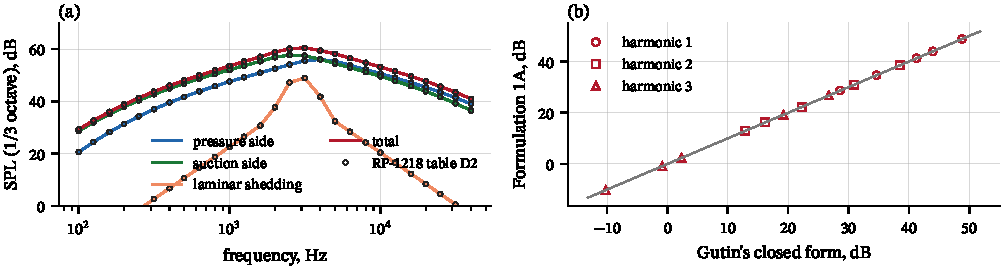
\includegraphics[width=\textwidth]{verify}
\caption{(a) The BPM port against the output of NASA's code; (b) Formulation 1A against Gutin's hover harmonics at five polar angles.}\label{fig:verify}
\end{figure*}
Table~\ref{tab:verify} and Fig.~\ref{fig:verify} show that the solvers do what they say. The port's error against table D2 is at the table's print precision; the tip column of table D3 differs by \NBpmTip\,dB where the tip lies 70\,dB under the total, which a 0.3\,\% different Strouhal number in the run that made the table explains. The test suite's \NTests{} tests pass.

\subsection{Rotor aerodynamics}\label{sec:rotor}
\begin{figure*}[t]
\centering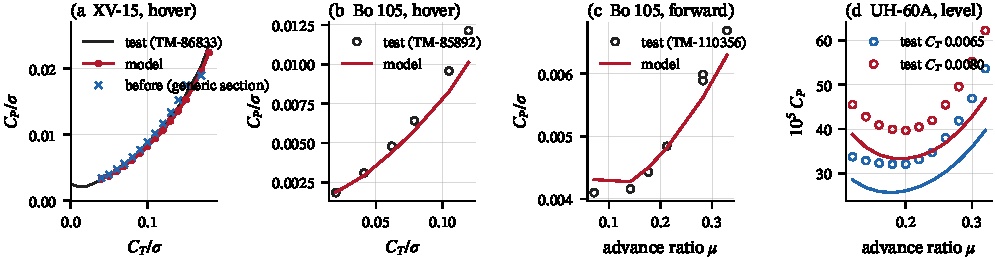
\includegraphics[width=\textwidth]{rotors}
\caption{Rotor power against tests: (a) the XV-15 rotor in hover, with what the trim returned for the generic section past its stall; (b, c) the Bo~105 rotor on NASA's stand and in its tunnel, $C_T/\sigma=0.07$, shaft 10$^\circ$ forward; (d) the UH-60A in level flight, both engines' output against both rotors' power.}\label{fig:rotors}
\end{figure*}
Fig.~\ref{fig:rotors} compares power. The XV-15 rotor is within \NXvCpMin{} to \NXvCpMax\,\% of its test over its whole range, as it should be with a section fitted to it. The Bo~105's is \NBoCpMax{} to \NBoCpMin\,\% from the test in the hover, falling short at high thrust; in the tunnel, shaft forward, \NBoFwdLo\,\% below $\mu=0.2$ and \NBoFwdHi\,\% above 0.27. The UH-60A's rotors are \NUhHoverMin{} to \NUhHoverMax\,\% from the engines' output in the hover, and in level flight \NUhLevelALo\,\% up to $\mu=0.24$ at $C_T=0.0065$ and \NUhLevelAHi\,\% above $\mu=0.28$. A few per cent of that is the transmission and accessories. The rest is not the rotor model at large, since the Bo~105 shows nothing like it at the same advance ratios; it may lie in the UH-60A's advancing tip, deep in the drag rise, or in its airframe's balance. It is not resolved. For the sound it matters less than it seems: the thrust is held and the loading noise follows the thrust, though the torque's share is low by as much.

\subsection{The elastic blade}\label{sec:blade}
\begin{figure*}[t]
\centering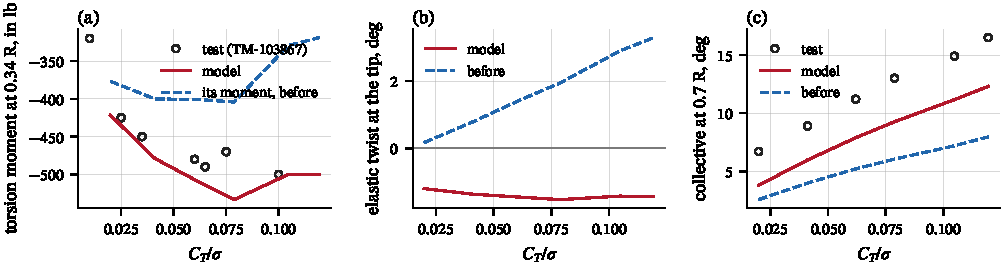
\includegraphics[width=\textwidth]{torsion}
\caption{The Bo~105's blade in hover, before and after the correction of its pitching moment: (a) the steady torsion moment at 0.34\,$R$ against NASA's; (b) the elastic twist at the tip; (c) collective at 0.7\,$R$.}\label{fig:torsion}
\end{figure*}
\begin{figure}[t]
\centering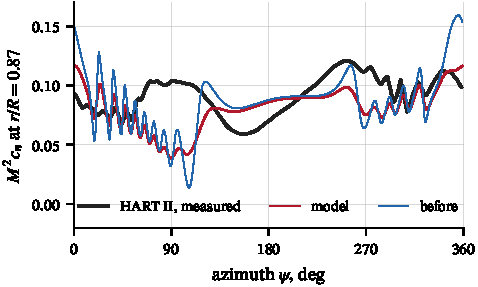
\includegraphics[width=\columnwidth]{hart2_loads}
\caption{HART~II baseline: section normal force at $r/R=0.87$.}\label{fig:hartloads}
\end{figure}
Fig.~\ref{fig:torsion} is the test that found the program's worst fault. The Bo~105's steady torsion moment at 0.34\,$R$ is within \NBoTorsMax\,\% of NASA's measurement at every thrust, nothing fitted, its three parts (the aerodynamic moment, the centrifugal force on the offset centre of mass, and the propeller moment) being each several times the difference between them. The blade twists \NBoTwistHi$^\circ$ at the tip at $C_T/\sigma=0.12$, where it twisted \NBoTwistBefore$^\circ$ before (Section~\ref{sec:review}). On HART~II's rotor the mean tip twist is \NHtTwist$^\circ$, the measured about $-1^\circ$~\cite{lim}; its flap at the tip runs from \NHtFlapLo{} to \NHtFlapHi\,m against a measured $-0.03$ to $+0.01$, the model missing the measurement's 2/rev. The collective stands \NBoThMin--\NBoThMax$^\circ$ under the test's, where it stood \NBoThBeforeMin--\NBoThBeforeMax$^\circ$; the flight model built on the blade's real distributions finds 2.5--3.1$^\circ$~\cite{bo105rep}, and the remainder here grows with thrust.

\subsection{Absolute level: the XV-15 rotor on NASA's stand}\label{sec:stand}
\begin{figure*}[t]
\centering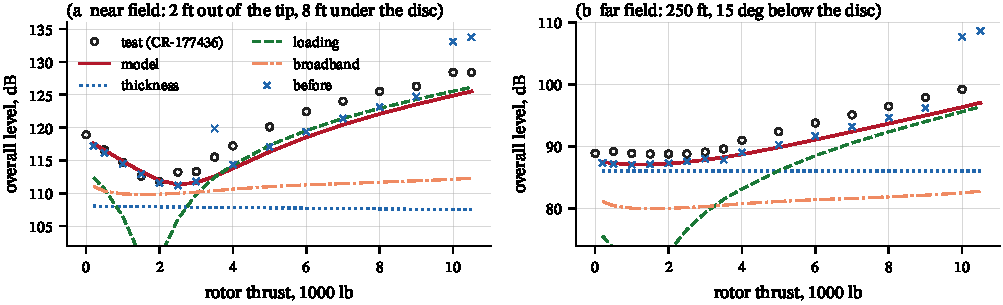
\includegraphics[width=\textwidth]{stand}
\caption{The full-scale XV-15 rotor's overall level against thrust on NASA's outdoor stand, tip Mach number 0.69, nothing fitted. Near field: the dip is where the tip's negative lift gives way, and the loading noise a microphone so close to the tip hears passes through a null.}\label{fig:stand}
\end{figure*}
This is the program's first absolute test of a rotor's level, and it uses no calibration at all: no wake passes close to a hovering blade. Fig.~\ref{fig:stand} gives the result. In the near field the model is \NStNearMean\,dB from the test on average, \NStNearRms\,dB rms, and at most \NStNearMax\,dB, from 200 to 10\,500\,lb. It finds the dip: \NStDipMod\,dB at \NStDipLb\,lb against the test's \NStDipTest\,dB at \NStDipTestLb\,lb. The blade's 36$^\circ$ of twist is why there is one. At low thrust its outer fifth carries negative lift, which only passes zero near \NStTipZero\,lb, and a microphone 2\,ft from the tip hears the tip first: the loading noise falls into a null as the tip unloads, adding to the thickness noise below it and cancelling it above, until the broadband is left. That near field is the one the MV-22B's cabin path rests on: the microphone was placed to stand for a tiltrotor's fuselage. In the far field the model is \NStFarMean\,dB from the test, \NStFarRms\,dB rms, the shape right; a microphone near the ground would read up to 6\,dB over the free field, so the offset may not be the model's. Before the XV-15 had its real section the same comparison gave \NStBeforeHi{} and \NStBeforeFar\,dB at 10\,000\,lb, against \NStTestHi{} and \NStTestFarHi: a trim failed in silence (Section~\ref{sec:review}).

\subsection{Blade--vortex interaction: HART~II}\label{sec:hart}
\begin{figure*}[t]
\centering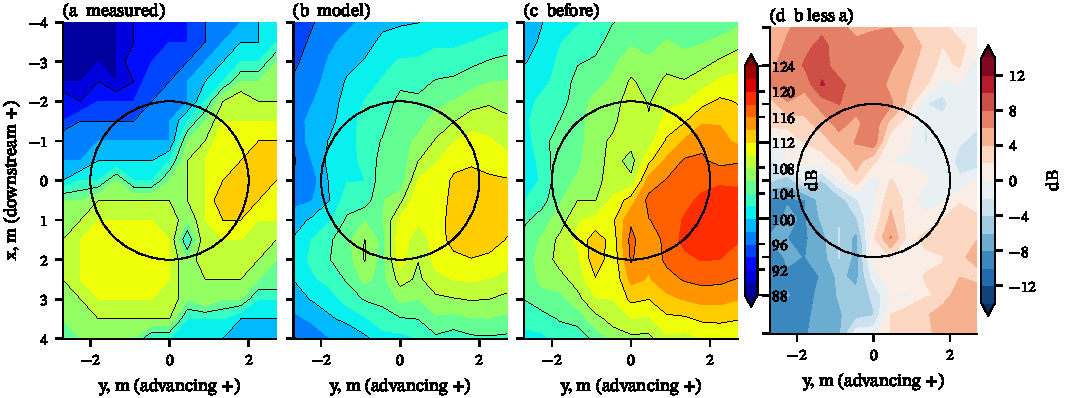
\includegraphics[width=\textwidth]{hart2_map}
\caption{HART~II baseline, 6--40 BPF level on the plane 2.215\,m under the hub: (a) measured~\cite{lim}, (b) the model, (c) the model before, (d) the model less the measurement. Flow from top to bottom is upstream to downstream; the circle is the disc.}\label{fig:hartmap}
\end{figure*}
\begin{table}[t]
\centering\small
\caption{HART~II baseline: the core's calibration. $\alpha_s$ in degrees, core in tip chords, rms of the load above 10/rev, the lobes' peaks, the map's mean error and scatter (dB) and its correlation with the measurement.}\label{tab:hart}
\resizebox{\columnwidth}{!}{\Tab{hart2}}
\end{table}
HART~II~\cite{lim} is the one rotor whose blade loads, deflections, wake and noise were all measured at one condition, at the maximum of its blade--vortex noise. With the rotor's published data the model gives a mean $M^2c_n$ of \NHtModMean{} against \NHtMean{} (Fig.~\ref{fig:hartloads}). Its impulsive part is another matter. A lifting line with the measured core, 0.12 chord, and all the circulation is \NHtMeasCoreRatio{} times too strong in the load above 10/rev and \NHtMeasCoreMean\,dB too loud over the plane. The real vortex is displaced and spread by the approaching blade, which a prescribed wake doesn't do: hence an effective core. It had been set at 0.4 chord to bring the UH-60A's and UH-1H's swings to ``about 0.1 in $M^2c_n$'', a figure taken for HART~II's swing that is in fact its mean: the swing is near \NHtRms{} rms. That left the program \NHtBeforeRatio{} times too strong in the load and \NHtBeforeMean\,dB too loud (Table~\ref{tab:hart}).

Calibrated on the noise itself, the core is \NHtCore{} chord. Fig.~\ref{fig:hartmap} shows the result. The mean error over the plane is \NHtMapMean\,dB by construction; what the calibration does not give is the rest. The scatter is \NHtMapRms\,dB and the correlation \NHtMapR, nearly the same at every core. Both lobes are there: the advancing one at \NHtAdvMod\,dB against \NHtAdv, a metre downstream of the measured one, and the retreating one in its place but \NHtRetDiff\,dB weak, \NHtRetMod{} against \NHtRet. The whole of this is the wake: without its impulses the plane's peak is \NHtNoBvi\,dB, \NHtBvidB\,dB down. The load's rms is still \NHtRmsRatio{} times the digitised measurement's, of which the thick line and the 2$^\circ$ reading take something. The prediction teams' own maps in the same paper, with free wakes and full comprehensive analyses, differ from the measurement by several decibels and from each other by as much~\cite{lim}, so this is about what the state of the art gives, at a small part of its cost, for a calibrated constant. Johnson's free-wake model of the V-22's scaled rotor uses a core of 20\,\% of the mean chord~\cite{wj}; the larger value here is the price of the prescribed wake.

\begin{figure*}[t]
\centering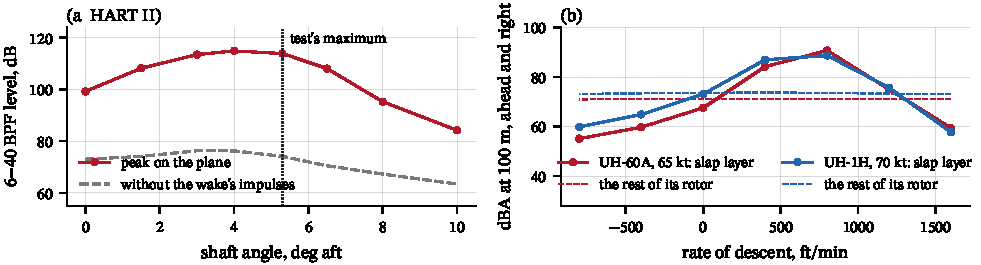
\includegraphics[width=\textwidth]{bvi}
\caption{(a) HART~II's noise against shaft angle: the test's baseline is at its maximum. (b) Slap against the rate of descent.}\label{fig:bvi}
\end{figure*}
The rest of the wake's behaviour needs no calibration: where the slap comes and goes. HART~II's baseline was set where the shaft-angle sweep found the maximum noise, 5.3$^\circ$; the model's maximum is at \NBvAlphaPeak$^\circ$ (Fig.~\ref{fig:bvi}a). In full-scale descents the slap peaks at \NBvUhFpm\,ft/min for the UH-60A at 65\,kt and \NBvHuFpm\,ft/min for the UH-1H at 70\,kt, with the wake in the disc's plane, and falls away in steeper descents as the wake rises through the disc (Fig.~\ref{fig:bvi}b).

\subsection{Absolute level in flight: the UH-60A}\label{sec:flight}
\begin{table}[t]
\centering\small
\caption{The UH-60A overhead: the FAA's measured maximum and the model's, dBA.}\label{tab:flight}
\Tab{flight}
\end{table}
\begin{figure*}[t]
\centering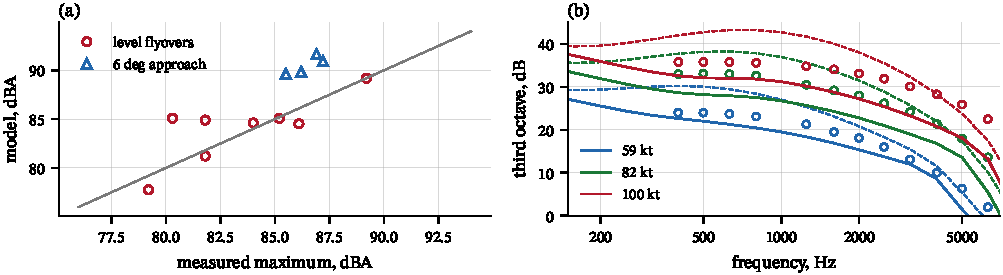
\includegraphics[width=\textwidth]{flight}
\caption{Absolute levels in flight, nothing fitted: (a) the UH-60A in the FAA's flyovers and approaches; (b) the ASK~21 model, lines, dashed with its fixed wheels, against the Prue-2 glider's smoothed bands, circles, at 59, 82 and 100\,kt.}\label{fig:flight}
\end{figure*}
The FAA flew a UH-60A over calibrated microphones in June 1980~\cite{faa}. Its appendices give every run's levels and a photograph's reading of the cockpit, so speeds and rates of descent need not be assumed. Table~\ref{tab:flight} and Fig.~\ref{fig:flight}a set the model against twelve sets of runs: the rotors and both engines at eight angles along the path, a microphone 1.2\,m over grass, the largest level taken. With nothing fitted the mean error is \NFlMean\,dB and the rms \NFlRms\,dB; the eight level flights have a mean of \NFlLevelMean\,dB and a scatter of \NFlLevelSd. Much the same flyover on two days differs by 1.9\,dB, which is what can be asked of it. The level follows the height from 91 to 305\,m, and the ground is right: a flush microphone reads \NFlFlushTest\,dB against the model's \NFlFlushMod, one 10\,m up \NFlTallTest{} against \NFlTallMod.

Speed is where it fails. From 100 to 152\,kt the test rises \NFlTestRise\,dB and the model \NFlModRise, from \NFlSlowDiff\,dB at 115\,kt to \NFlFastDiff\,dB at 152. Power isn't the reason: against the torque the crew read, the model's is \NFlTorqueLo{} to \NFlTorqueHi\,\% at every speed and rises as the test's does. The test's overall level rises \NFlOaRise\,dB, more than its A-weighted one, so what grows with speed is low in pitch, and the model hasn't got it.

Four approaches down the 6$^\circ$ path, at 56 to 76\,kt, read \NFlAppTestLo{} to \NFlAppTestHi\,dBA and the model \NFlAppLo{} to \NFlAppHi, \NFlAppMin{} to \NFlAppMax\,dB over: high, but evenly, with the torque at 20 to 25\,\% where the crews read 17 to 35. The slap alone comes to \NFlAppSlap\,dBA, against \NFlLevelSlap{} at most in level flight, and the rest to \NFlAppRest, so not all of the excess can be the slap's, and a maximum level does not separate them. A vortex core set on a 40\,\% scale rotor in a wind tunnel has at least not put a full-scale aircraft's slap far out.

Beside the path the model is plainly wrong. On one day's flyovers at 150\,kt and 152\,m, microphones 150 and 164\,m to the side read \NFlNearTest\,dB from the one under the path, and one 284\,m out \NFlFarTest; the model gives \NFlNearMod{} and \NFlFarMod, \NFlSideLo{} to \NFlSideHi\,dB short. Its main rotor's broadband leads everywhere and simply fades with distance, where the real sound is stronger sideways than downward. The overall level stands \NFlGapCentre\,dB over the A-weighted one under the path and \NFlGapSide{} beside it, so what is missing there is higher in pitch than what is missing with speed; the tail rotor is the likely place, but with no spectra that is a guess, and nothing has been fitted to it.

\subsection{Texture}\label{sec:texture}
\begin{table}[t]
\centering\small
\caption{Loops against recordings: how alike consecutive blade passages are, the harmonics against the noise from 100\,Hz to 3\,kHz, and the crest factor. In brackets, the same render without the unsteadiness.}\label{tab:texture}
\resizebox{\columnwidth}{!}{\Tab{texture}}
\end{table}
\begin{figure}[t]
\centering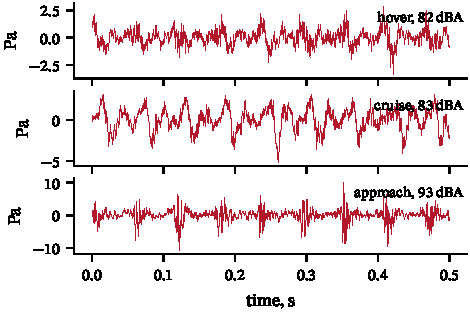
\includegraphics[width=\columnwidth]{texture}
\caption{UH-60A loops at 100\,m: half a second of a hover, a cruise and an approach.}\label{fig:texture}
\end{figure}
A loop can have the right spectrum and sound like nothing that flies. Table~\ref{tab:texture} shows the measures that told the first loops from recordings. Consecutive blade passages in the recordings correlate at \NTxRecLo--\NTxRecHi, in a perfectly periodic render up to \NTxSteady, and with the unsteadiness at \NTxModLo--\NTxModHi. An approach is \NTxApproach\,dBA over a cruise for the same listener (Fig.~\ref{fig:texture}), where it was $+25$ in the first loops and \NTxApproachBefore{} with the previous core.

\subsection{Tiltrotors outside}\label{sec:outside}
\begin{figure}[t]
\centering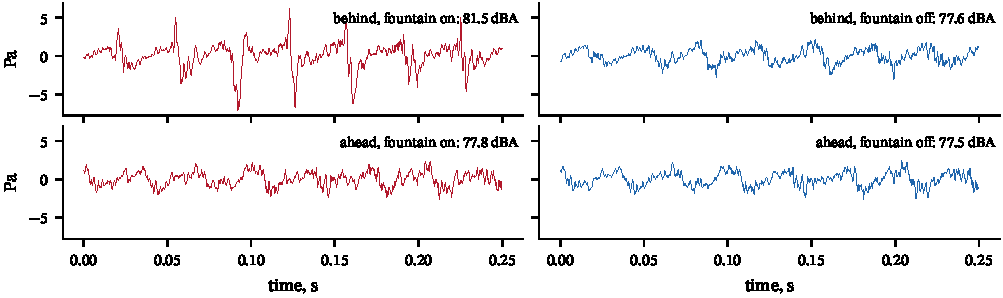
\includegraphics[width=\columnwidth]{fountain}
\caption{XV-15 hovering over a ground board at 57 radii, 46$^\circ$ below the disc.}\label{fig:fountain}
\end{figure}
\begin{table}[t]
\centering\small
\caption{MV-22 in a hover: published maxima and the model's rotors, fast response, hard ground, dBA.}\label{tab:outside}
\Tab{outside}
\end{table}
\begin{figure}[t]
\centering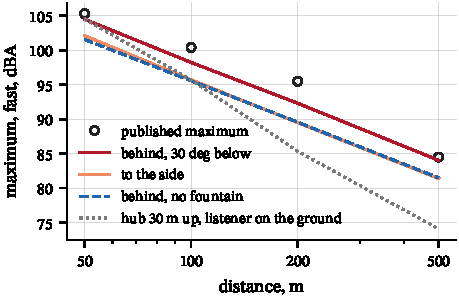
\includegraphics[width=\columnwidth]{outside}
\caption{MV-22 hover levels against distance.}\label{fig:outside}
\end{figure}
A hovering tiltrotor is louder behind than to the side, which surprised NASA in 1981 and which George explained by the fountain's reingestion~\cite{ma}. The model has the same asymmetry from the same cause (Fig.~\ref{fig:fountain}). At 57 radii on a ground board the wave ahead is about \NFoAheadPa\,Pa, as measured~\cite{rcg}, with no spikes; behind, spikes reach \NFoSpikeC\,Pa at 46$^\circ$ below the disc, measured about 15, and \NFoSpikeA--\NFoSpikeB\,Pa at 13$^\circ$ and 23$^\circ$, measured 5: too strong by up to a factor of two near the disc's plane and too weak well below it. The fountain adds \NFoBehind\,dBA behind and \NFoAhead{} ahead; fences that removed it took \NFoFences\,dBA off~\cite{george}.

Table~\ref{tab:outside} and Fig.~\ref{fig:outside} set the MV-22's rotors against the published maxima~\cite{mod}. Behind the aircraft, 30$^\circ$ below the disc, over hard ground at fast response, they are within \NOuBehindMax\,dB, nothing fitted; the fountain gives \NOuFountain\,dB of that. Since the table doesn't say where its microphones were, this shows that a reasonable geometry reproduces it, no more; a low hover heard along the ground falls away too fast to fit. In airplane mode at 220\,kt directly below, the model makes \NOuBelow\,dBA at 100\,m, which spreading alone takes to \NOuSpreadA, \NOuSpreadB{} and \NOuSpreadC\,dBA at 500, 1000 and 1500\,ft against 88, 81 and 78; without the wing it made \NOuBelowNoWing.

\subsection{Turbine engines}\label{sec:engines}
\begin{figure*}[t]
\centering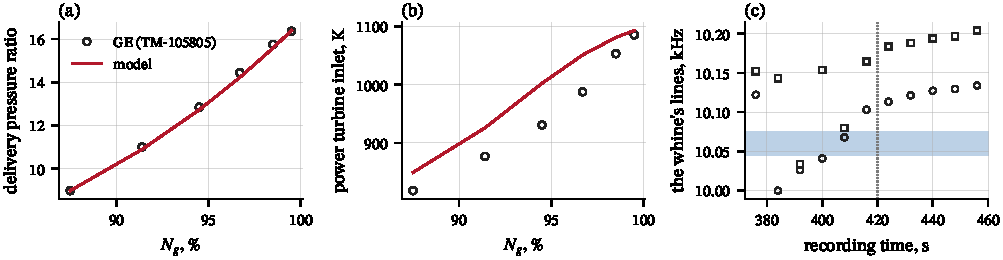
\includegraphics[width=\textwidth]{engines}
\caption{(a, b) The T700's cycle against GE's simulation. (c) The two whine lines in a UH-60's recording, drifting up through the $\pm 15$\,Hz window (shaded) in which an earlier check read them, at the moment (dotted) it took for the doors closing.}\label{fig:engines}
\end{figure*}
The T700's cycle follows GE's simulation within \NEnPr\,\% in delivery pressure and \NEnTemp\,K in power turbine inlet temperature, hot where GenHel's fuel flow, which the flight model uses, runs about 5\,\% over GE's (Fig.~\ref{fig:engines}). The AE~1107C's published design point is met by construction: \NEnAeFlow\,kg/s and \NEnAeTemp\,$^\circ$C against 15.9 and 1209.

Tones are where recordings are at their best, since frequency survives any camera. A UH-60M's whine at idle settles on two lines at \NToIdleA{} and \NToIdleB\,kHz, in the ratio \NToRatio: exactly 10:11, which gives its first two stages 20 and 22 blades at \NToNgIdle\,\% $N_g$. The same whine sits at \NToFly\,kHz on the ground at FLY and \NToHover\,kHz in the hover (\NToNgFly{} and \NToNgHover\,\%). The gearbox's planetary mesh stands at \NGeHz\,Hz, its line growing \NGeRise\,dB over the floor beside it from flat pitch to the hover, where its amplitude's following the torque gives \NGeModel\,dB: the mesh depends on its load more steeply than that, or at flat pitch it isn't heard at all, which a line 3\,dB over its floor can't tell.

Outside, 50\,m to the right, one T700 makes \NEnIdle\,dBA at idle, \NEnFly{} at 87.5\,\% and \NEnFull{} at full power, and the APU \NEnApu, against 85\,dBA contours past 100\,ft and levels of 105\,dB or more measured round a whole UH-60 on the ground~\cite{jones}. GE's and Heidmann's methods are empirical and good to about 5\,dB.

\begin{figure*}[t]
\centering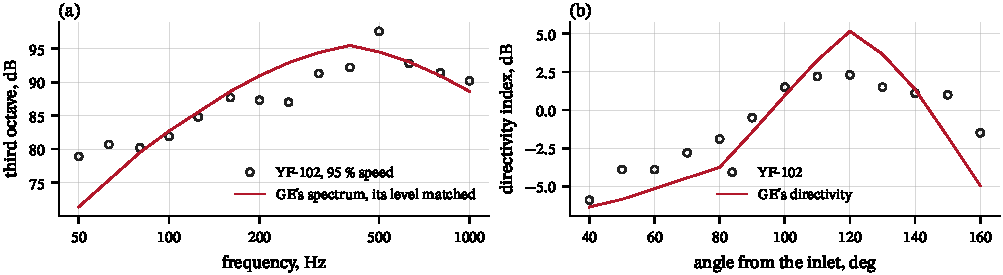
\includegraphics[width=\textwidth]{combustion}
\caption{GE's combustion noise against a YF-102, a turbofan on a helicopter's core: (a) the spectrum's shape against the core noise at 95\,\% speed, 120$^\circ$ from the inlet~\cite{krejsa}; (b) the directivity against the coherent noise from 30 to 60\,\% speed~\cite{karchmer}.}\label{fig:combustion}
\end{figure*}
Combustion noise can be tested on its own, because NASA separated it on a YF-102, a turbofan built on the core of a helicopter's T55. GE's published power for that engine~\cite{karchmer}, by the method used here, stands \NCoDirectLo{} to \NCoDirectHi\,dB over its far field below 200\,Hz, which bounds it from above, and \NCoCohLo{} to \NCoCohHi\,dB over the part coherent with one combustor probe, which Krejsa shows reads 3 to 10\,dB low~\cite{krejsa}: about right, on the high side. Those are GE's own figures, since these reports don't give the engine's cycle; the port rests on ANOPP's equations. Its spectrum's shape follows the core noise found by Krejsa's three signals within \NCoShape\,dB rms, peaking at \NCoPeak\,Hz against the method's 400, and its directivity follows the measured within \NCoDi\,dB rms, \NCoDiMax\,dB at most (Fig.~\ref{fig:combustion}). The single probe had put that peak near 125\,Hz at lower power, which, taken alone, would have argued for moving the spectrum two octaves down; the better measurement doesn't. Modern engines are another matter: flight tests put the method \NCoModLo{} to \NCoModHi\,dB over a GEnx-1B and a GE90~\cite{nesbitt}, whose pressure ratios and combustors are far from a T700's. The doubt costs little here, since the power turbine leads: 10\,dB off a T700's combustion noise takes \NCoCutLo{} to \NCoCutHi\,dB off the engine 50\,m away. The jet's power by SAE's method stands \NCoJetLo{} to \NCoJetHi\,dB over NACA's constant for cold jets and engines alike~\cite{naca}, and the spectrum's peak, which stood at a Strouhal number of 0.5, now stands at \NCoJetSt, as NACA measured it, 0.3. A turboshaft's slow jet lies some 20\,dB under its combustion noise, so neither is heard.

\subsection{Cabins and wind}\label{sec:cabin}
\begin{figure}[t]
\centering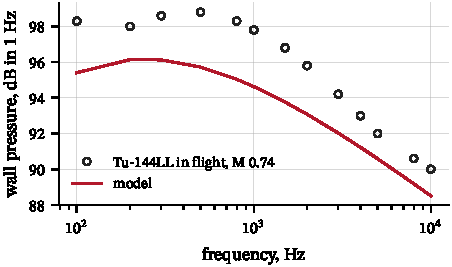
\includegraphics[width=\columnwidth]{wind}
\caption{The boundary layer's wall pressure in flight~\cite{tu144}.}\label{fig:wind}
\end{figure}
\begin{figure*}[t]
\centering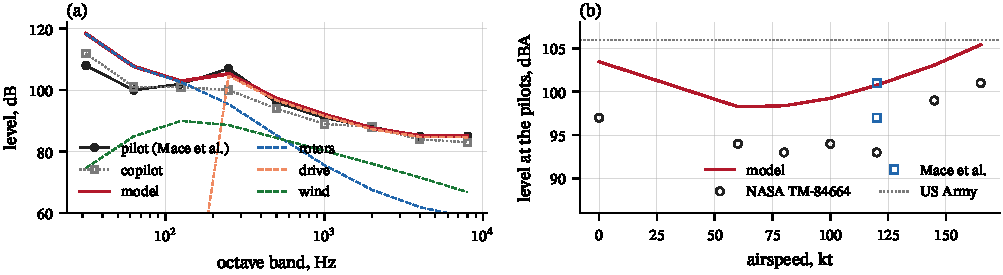
\includegraphics[width=\textwidth]{cockpit}
\caption{The UH-60A at the pilots: (a) octave bands at 120\,kt, the model calibrated on the pilot's above 125\,Hz; (b) level against airspeed, NASA's data independent of that calibration.}\label{fig:cockpit}
\end{figure*}
\begin{figure*}[t]
\centering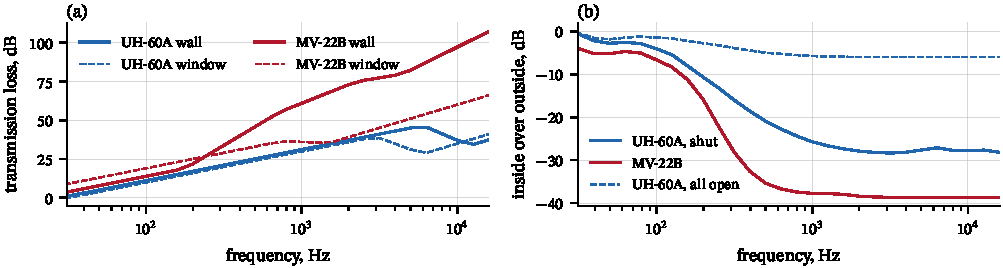
\includegraphics[width=\textwidth]{cabin}
\caption{(a) Transmission loss of the walls and windows; (b) what reaches the listener of what is outside.}\label{fig:cabin}
\end{figure*}
Fig.~\ref{fig:cabin} shows the walls: the MV-22B's double wall far tighter than one wall above its resonance at \NCaResonance\,Hz, and the windows' coincidence dips. Opening every door and window of the UH-60A adds \NCaDoor\,dB to the path at 10\,kHz, a figure with no measurement behind it now (Section~\ref{sec:review}). That is the one part of the UH-60A's cabin left without a measurement, for its cockpit now has several (Fig.~\ref{fig:cockpit}). Mace's survey gives the octave bands at the pilot's seat at 120\,kt, doors shut~\cite{usaarl}. Against it the first model was right in total for the wrong reasons: \NCkOldCruise\,dBA, but its gearbox, set from NASA's review~\cite{review}, stood \NCkOldTone\,dB over the 1\,kHz octave and the other bands from 250\,Hz to 8\,kHz \NCkOldUnderLo{} to \NCkOldUnderHi\,dB under, with no wind in the preset and none of the drive's vibration through the airframe. With the wind added, the tones taken down and what remains measured as the drive's bands, as for the MV-22B, the model is within \NCkBandMax\,dB of that spectrum from 125\,Hz up, which is a calibration, and \NCkCruise\,dBA against \NCkPilot. Below 100\,Hz it stands \NCkLowLo{} to \NCkLowHi\,dB over: this fuselage has no wall model, so the rotors' harmonics pass the cabin filter whole. NASA's levels~\cite{tm84664}, independent of that calibration, show what it is worth: from the hover to 165\,kt the model runs \NCkNasaMean\,dB over them but follows their trend with speed within \NCkNasaSd\,dB (the drive with the torque, the wind with the speed). The model's hover, \NCkHover\,dBA, lies between NASA's \NCkNasaHover{} and the Army's \NCkArmy~\cite{nas}. The wall pressure lies at \NWiLo--\NWiHi\,$q$ over the flight range, against Bies's compilation of flight and tunnel data, about 0.0066\,$q$~\cite{bies}. In flight the Tu-144LL measured it in absolute terms~\cite{tu144}: at Mach 0.74 and 16\,400\,ft, mid-fuselage, the model's spectrum keeps the measured shape within \NWiTuShape\,dB rms from 100\,Hz to 10\,kHz, closer than the five established models that report tried, and is \NWiTuMean\,dB in level (Fig.~\ref{fig:wind}), at \NWiTuQ\,$q$. That run's Reynolds number, $3\times10^8$, is far past what the 1/7-power skin friction used until then can reach, which stood 4.8\,dB under; White's law takes half of that. The rest isn't explained, the sensors themselves scattering by about 1.5\,dB and the model leaving out compressibility. The wind's altitude scaling holds the spectrum from 125\,Hz to 2\,kHz within \NWiAltA\,dB to 12\,km and \NWiAltB\,dB at 21\,km, and is \NWiAltTop\,dB out at 16\,kHz there.

\subsection{The MV-22B's cockpit}\label{sec:mv22}
\begin{figure*}[t]
\centering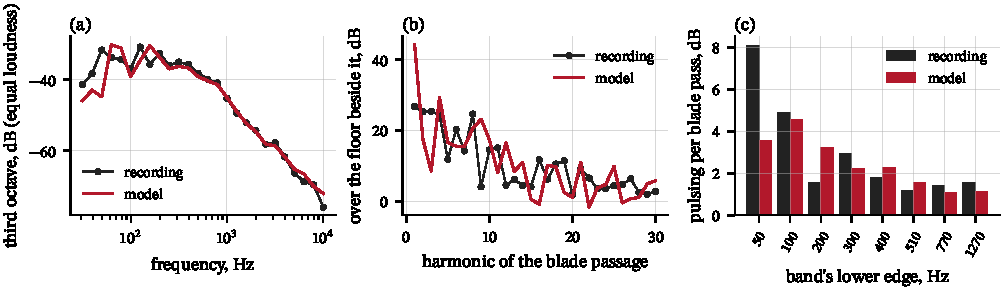
\includegraphics[width=\textwidth]{mv22}
\caption{MV-22B in cruise behind the pilots, model against recording at equal loudness: (a) third octaves; (b) each blade harmonic over the broadband beside it; (c) how hard each band pulses with the blades.}\label{fig:mv22}
\end{figure*}
\begin{table}[t]
\centering\small
\caption{MV-22B cockpit: recording and model.}\label{tab:mv22}
\Tab{mv22}
\end{table}
\begin{table}[t]
\centering\small
\caption{Each term of the proprotors' path taken out: their level, harmonics over the floor (dB), the 100--200\,Hz band's pulsing (dB) and line share (\%).}\label{tab:terms}
\resizebox{\columnwidth}{!}{\Tab{terms}}
\end{table}
A public video of an MV-22B in airplane-mode cruise has a camera behind the pilots for two and a half minutes and at a cabin window beside a nacelle for as long. The proprotors pass their blades at \NMvBpf\,Hz (\NMvRpm\,rpm, the preset's airplane mode). At the window the first compressor stage's whine stands at \NMvWhine\,kHz and falls to \NMvWhineOff\,kHz as the power comes off; 32 blades put it there at the flight model's 90.5\,\% $n_1$. It is chopped by the proprotor, its line's envelope \NMvChop\,dB over its floor at the blade rate where the broadband beside it shows \NMvChopBeside: the model doesn't have this.

This comparison took the most work, and the least of it is prediction. Heard at the listener's head through limp walls the model was the proprotors' first harmonics with little else, ``a wind tunnel'' to the ear that compared them. What the recording has besides is a steady roar from 40\,Hz to 12\,kHz, strongest by the wing's root: the drive's and engines' vibration through the wing and the frames, which cannot be computed and is measured. The proprotors' harmonics from the 6th to the 30th stand far out of that roar, 0.75\,dB a harmonic down, where a blade's own pressure falls 2.4; the wing behind the discs makes them, and through the structure its loads fall 0.9\,dB a harmonic as the recording's do. What remains after these terms is in Table~\ref{tab:mv22} and Fig.~\ref{fig:mv22}: at equal loudness the model is within \NMvBand\,dB in every octave-wide band from 50\,Hz to 12\,kHz (\NMvLow\,dB under at 25--50\,Hz, where the camera's response is unknown). Third octaves agree within \NMvThirdMid\,dB from 200\,Hz to 5\,kHz; below that a band holds one or two harmonics, and which of them stand on the cabin's resonances is a draw, so they differ by up to \NMvThirdLow\,dB. The floor between the lines within \NMvFloor\,dB from 39 to 500\,Hz but for one third octave. The proprotors make \NMvRotors\,dBA, the drive \NMvDrive, the wind \NMvWind{} and the engines \NMvEngines, \NMvAll\,dBA in all at the camera. That absolute figure is not a measurement: the drive's level is set from the recording relative to the proprotors, so it rests on them. Table~\ref{tab:terms} shows that each term earns its place: without the wing the harmonics from the 14th fall into the floor and those from the 6th lose half their height; with the rotors in step the low ones stand 4\,dB over the recording's; and in sea-level air the surface layer's turbulence buries them. The trim wall changes the proprotors least; its work is on the wind, which this table holds fixed. Those statistics were matched with the parameters listed in Table~\ref{tab:params}, so the table shows how consistent the physics is with one recording, not that it predicts one.

\subsection{The ASK~21}\label{sec:ask21}
\begin{figure*}[t]
\centering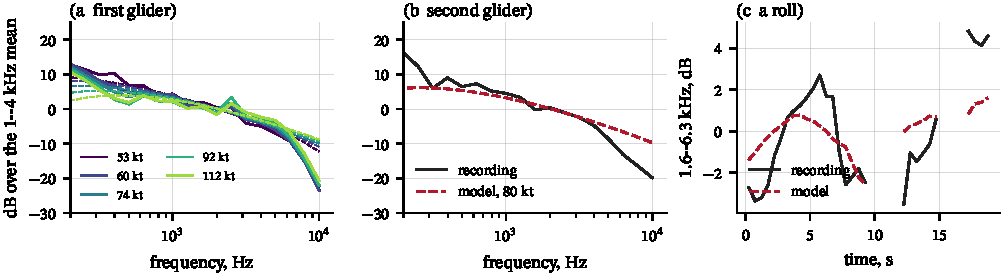
\includegraphics[width=\textwidth]{ask21}
\caption{ASK~21 cockpits: (a) spectra by airspeed, solid the recording and dashed the model, each set to its 1--4\,kHz mean; (b) a second glider; (c) a barrelled roll, the 1.6--6.3\,kHz band, in the stretches where the ASI reads.}\label{fig:ask21}
\end{figure*}
The computed stall speed at 540\,kg is \NAsStall\,kt, the flight manual's 35. Outside, NASA's flyovers of a Prue-2 glider~\cite{healy} give the first absolute test. Healy smoothed their spectra, leaving out the tones and the ambient below about 300\,Hz. At the same height and speeds the ASK~21 model, its wheels left out, has their shape within \NPrShape\,dB rms from 400\,Hz to 6.3\,kHz at each speed, and stands \NPrLo{} to \NPrHi\,dB under them (Fig.~\ref{fig:flight}b). Its overall level goes as $V^{\NPrExpModel}$ and theirs as $V^{\NPrExpTest}$. Healy's law, $M^6S/AR^4$ fitted to all his aircraft, puts an ASK~21 within \NPrLawMean\,dB of the Prue-2's level, so wing size and aspect ratio do not excuse the difference, and the model stands \NPrLawModel\,dB from that law. Whether the rest is the type's finish or a source the model lacks cannot be told from another glider. In the cockpit the canopy's boundary layer dominates, \NAsLevelLo\,dBA at 50\,kt and \NAsLevelHi{} at 120\,kt. In aerobatics recorded from the front seat, airspeed read off the needle frame by frame, the shape from 315\,Hz to 6.3\,kHz is within \NAsShapeLo--\NAsShapeHi\,dB rms at \NAsSpeedLo{} to \NAsSpeedHi\,kt (Fig.~\ref{fig:ask21}a), and from 400\,Hz to 8\,kHz, without the bands a whistle of this glider's own crosses, the sound's power grows as the airspeed to the power \NAsExpRec, the model's \NAsExpMod; from 3 to 8\,kHz it grows \NAsHighRec\,dB a decade against \NAsHighMod. A second glider, \NAsSecondSec\,s free of the music's cymbals, keeps the shape within \NAsSecond\,dB from 400\,Hz to 4\,kHz. Both fall faster than the model above 5\,kHz; how much of that their cameras make can't be told. In a barrelled roll with the load factor read off the g-meter, the band swings \NAsRollRec\,dB against the model's \NAsRollMod, the same way, and in the pull-up grows \NAsPerGRec\,dB per $g$ against \NAsPerGMod. Leaks through the canopy's seals, driven by the lift and the slip, would do this. So might the camera, and one recording can't tell them apart.

The Prue-2 comparison leaves out a source the ASK~21 has: its wheels don't retract. By Fink's method~\cite{anopp}, taking a wheel that stands out of the belly, with its image in the belly, as a body of twice that height, they add \NWhLo{} to \NWhHi\,dB outside from 400\,Hz to 1\,kHz, peaking near \NWhFLo\,Hz at 59\,kt and \NWhFHi\,Hz at 100 (dashed in Fig.~\ref{fig:flight}b), which would put an ASK~21 \NWhVsPrue\,dB over the Prue-2 at 59\,kt and 400\,Hz; Healy doesn't say whether the Prue-2's wheel was up. The method can be checked in the same test on a Cessna~150 with bare wheels: its wheels alone come to \NWhCeLo{} to \NWhCeHi\,dB under the whole aircraft, as they should. The image and the smaller tyres' sizes are estimates, good to perhaps 5\,dB, and no measurement of an ASK~21 outside exists to test them. In the cockpit the wheels' sound through the air stays \NWhInHi{} to \NWhInLo\,dB under the wind, and changes the comparison above by under 0.1\,dB. So it doesn't explain what the recordings have below 300\,Hz.

Those low bands need care. Split band by band into a part that follows the airspeed and a part that doesn't, the aerobatics recording holds a fixed floor of \NRoFloorLo{} to \NRoFloorHi\,dB up to 126\,Hz (set, like everything here, to the model's 1--4\,kHz). At 32, 40 and 79\,Hz it is all there is: the level at a stall turn's 35\,kt is within \NRoFlat\,dB of that at 115\,kt. That is not the flow, so it isn't modelled; the camera is the likely cause, and taken for a sound of the air it would have put a drone in the cockpit that doesn't fade at the stall. What does follow the airspeed, about as its cube, stands \NRoOverLo{} to \NRoOverHi\,dB over the model from 126 to 251\,Hz and joins it by 400\,Hz. This is taken as measured: the cockpit's low roar, a table of bands from 50 to 316\,Hz growing as $V^3$, with the rest of the model's bands untouched. It brings that recording within \NRoFitLo{} to \NRoFitHi\,dB rms from 126 to 316\,Hz, which shows only that the fit worked. The test is the roll: a phone on a pilot's head in another glider, not used for it, goes from \NRoRollWithoutLo--\NRoRollWithoutHi\,dB rms to \NRoRollWithLo--\NRoRollWithHi. The second glider's video has music under it and isn't used. What makes the roar is not known: the main wheel is bolted to the shell under the seat, and the fuselage's own skin is another candidate.

\subsection{Cost}\label{sec:cost}
On an Apple M1 (8 cores), busy with other work during this run (a load average of \NBeLoad, which about doubles these times), the source-time, closed-form kernel takes \NBeSrc\,ms where the classic retarded-time iteration, as the original WOPWOP does it, with the same compiler, takes \NBeRet\,ms, \NBeRatio{} times as long for the same answer. A UH-60A descent's trim, elastic response and wake take \NBeTrim\,s, Formulation 1A at one listener \NBeFa\,s (\NBeRate{} million source evaluations a second), and a whole 15\,s loop from nothing \NBeLoop\,s. PSU-WOPWOP itself was not timed: its binary is distributed on request, so no ratio is claimed.

% =====================================================================================================================
\section{Corrections found during validation}\label{sec:review}
\begin{table}[t]
\centering\small
\caption{What this report's corrections changed.}\label{tab:before}
\resizebox{\columnwidth}{!}{\Tab{before}}
\end{table}
The changes the comparisons forced are listed because each removed a physical, numerical or measuring error rather than tuning a coefficient. The first eight were found by this report's programme (Table~\ref{tab:before}).
\begin{enumerate}
\item \emph{The blades' pitching moment.} The section's moment about the elastic axis was the dynamic pressure, which held one chord already, times the chord squared: one chord too many, in metres. So the Bo~105's aerodynamic moment was 27\,\% of its value and the centrifugal term won: the blade twisted nose-up with thrust by \NBoTwistBefore$^\circ$, where NASA measured nose-down moments. Every elastic rotor had it, and every check passed, since the trim absorbs a twist in the collective. Comparing the moment with its three parts' sum found it, within 0.01$^\circ$.
\item \emph{The propeller moment} on the set pitch was missing from the torsion load.
\item \emph{A trim that failed in silence.} After 80 iterations the trim returned whatever it had. The XV-15's generic smooth section stalled so abruptly that the rotor could not make $C_T/\sigma$ of 0.16, and what came back had \NXvFalse{} times the power, \NStBeforeHi{} and \NStBeforeFar\,dB at the stand's microphones where the test has \NStTestHi{} and \NStTestFarHi. The Bo~105 at $\mu=0.33$ had no such excuse: nearly converged, a stale Jacobian and the lagging elastic state threw the iteration out, and it marched to 90$^\circ$ of cyclic and 14 times the power (this with the moment of item~1 corrected; the old blade happened to converge there). The trim now falls back to its best point in smaller steps, and stops with an error if it can't reach its thrust. Of 43 conditions that had converged, none moved at all. The XV-15 has the V-22 model's 64-series table.
\item \emph{The vortex core's target.} Section~\ref{sec:hart}: it had been aimed at a mean taken for a swing, and on other rotors than HART~II's.
\item \emph{A door check that wasn't.} Closing a UH-60's cabin doors in a recording was said to take 18.3\,dB off the whine at 10\,kHz, within a decibel of the walls' model. The figure came from one line in a $\pm 15$\,Hz window. In fact the two engines' lines drift from \NDoFromA{} to \NDoToA\,kHz through that moment at constant level (Fig.~\ref{fig:engines}c): the band's power changes \NDoBand\,dB, the window's \NDoNarrow. The check is withdrawn; nothing in the recording shows a door.
\item \emph{The skin friction.} The wall pressure's 1/7-power law falls short past $Re_x=10^7$. The Tu-144LL's flight spectra, whose shape the model had right, stood 4.8\,dB over it; White's law takes half of that, and 1 to 2\,dB more of wind on an MV-22B.
\item \emph{The UH-60A's cockpit, right for the wrong reasons.} Its gearbox tone, set from a review of such cabins, was \NCkOldTone\,dB too strong, and the cockpit had no wind and no broadband drive; the total was close only because these cancelled. A calibrated spectrum showed it (Section~\ref{sec:cabin}).
\item \emph{The HART~II map, read upside down} at first by this report's author, which correlated at 0.25 and was corrected from the paper's text (Section~\ref{sec:ref}), not from that correlation.
\item \emph{Perfect periodicity.} The first loops' passages correlated at 0.99 against the recordings' 0.2--0.6, with tones 12 to 17\,dB too strong. Hence the revolutions of their own and the blade-wake noise.
\item \emph{Sea-level air in a cruise at 10\,000\,ft} made every rotor pressure 2.6\,dB too strong, and the near-ground turbulence an inflow rumble as strong as the harmonics.
\item \emph{True for calibrated airspeed.} A simulator fades by calibrated airspeed, so a bank flying the same figure as true airspeed at altitude fell 4\,dB short.
\item \emph{The canopy's 30\,dB leak cap}, assumed for a glider's seals, left the cockpit flat from 2\,kHz up, 6 to 8\,dB too bright. Recordings removed it.
\item \emph{The rotors in step.} Below the cabin's lowest mode their pressures add coherently; in step the MV-22B's second harmonic stood 12\,dB too strong.
\item \emph{Beating.} With equal levels neighbouring harmonics beat, and a band pulsed 14\,dB a blade pass where the recording's pulses 5. The cabin's modal response removed it.
\item \emph{An A-weighted level match} made an A/B comparison sound nothing alike. Equal loudness by BS.1770 is what a listener compares.
\item \emph{A coarse blade-passing frequency.} Fitting it from the first harmonic at 0.18\,Hz resolution missed every line above the 12th; the recording's over-floor numbers had to be redone from the 6th to the 25th lines.
\item \emph{The gearbox's fade} ended at the helicopter mode's rotor speed, taking 1.5\,dB off in cruise at 83.7\,\%.
\end{enumerate}

% =====================================================================================================================
\section{Assessment}\label{sec:assess}
\begin{table}[t]
\centering\small
\caption{Summary: \ok{} within the data's scatter, \pok{} partly, \nok{} not reproduced. (P) a prediction, (C) calibrated on it, (M) parameters measured from it.}\label{tab:score}
\begin{tabularx}{\columnwidth}{@{}>{\raggedright\arraybackslash}Xc@{}}
\toprule
Solvers against closed forms and NASA's BPM code (P) & \ok \\
XV-15 rotor hover power (section fitted) & \ok \\
Bo~105 hover power (P) & \pok \\
Bo~105 forward-flight power (P) & \ok \\
UH-60A level-flight power at high speed (P) & \nok \\
Bo~105 torsion moment (P) & \ok \\
HART~II tip twist (P) & \ok \\
Bo~105 collective (P) & \pok \\
XV-15 near-field level against thrust (P) & \ok \\
XV-15 far-field level against thrust (P) & \ok \\
HART~II noise: mean (C) & \ok \\
HART~II noise: lobes and map (P) & \pok \\
HART~II load above 10/rev (C) & \pok \\
Pass-to-pass texture (assumed unsteadiness) & \ok \\
XV-15 fountain: behind and ahead (P) & \ok \\
XV-15 fountain spikes at shallow angles (P) & \pok \\
Wall pressure in flight: shape (P) & \ok \\
Wall pressure in flight: level (P) & \pok \\
MV-22 hover table (P, geometry unknown) & \pok \\
MV-22 airplane mode below (P) & \ok \\
T700 cycle (P) & \ok \\
Turbine tones' frequencies (M) & \ok \\
Combustion noise: shape, directivity (P) & \ok \\
Combustion noise: level (GE's figures) & \pok \\
Gearbox tone against torque (P) & \nok \\
UH-60A under its path, against height (P) & \ok \\
UH-60A under its path, against speed (P) & \nok \\
UH-60A in approach (core from HART~II) & \pok \\
UH-60A beside its path (P) & \nok \\
UH-60A torque in flight and approach (P) & \pok \\
Ground and microphone height (P) & \ok \\
UH-60A cockpit spectrum over 125\,Hz (M) & \ok \\
UH-60A cockpit under 100\,Hz (P) & \nok \\
UH-60A cockpit level, trend with speed (P) & \ok \\
UH-60A cockpit level against NASA's (M) & \pok \\
A glider's spectrum outside, another type (P) & \ok \\
A glider's level outside, another type (P) & \pok \\
Fink's wheels on a Cessna~150 (P) & \ok \\
A glider's fixed wheels outside & not tested \\
Cabin doors & not tested \\
Whine chopped by the proprotor & not modelled \\
MV-22B cockpit shape and statistics (M) & \ok \\
ASK~21 cockpit shape, 315\,Hz--6.3\,kHz (P) & \ok \\
ASK~21 above 5\,kHz (P) & \nok \\
ASK~21 from 126 to 316\,Hz, on another glider (M) & \pok \\
ASK~21 hiss against load factor (P) & \nok \\
\bottomrule
\end{tabularx}
\end{table}
Table~\ref{tab:score} summarises. The core of the program, from a rotor's published data to the pressure at a microphone, is now tested in absolute decibels, and it holds: on a full-scale rotor with nothing fitted, near and far, and on the elastic blade's moments. Blade--vortex interaction needs one calibrated constant and then reproduces the level, the lobes and the trends of the one test that measured them all. And under the flight path it holds in flight: a real UH-60A's level from 91 to 305\,m comes out with a scatter of \NFlLevelSd\,dB with no fitting, and a glider of another type keeps its spectrum's shape, \NPrLo{} to \NPrHi\,dB low. These are the program's strongest results, and they are also its newest: none of them existed before this report, and two of the faults they found had been passing every check for days.

Its weakest results are those that sound the most convincing. The MV-22B's cockpit agrees with its recording because many of its parameters were measured from that recording, by a camera of unknown response in one flight condition. The UH-60A's cockpit is calibrated on one survey that others differ from by 8\,dB, and the MV-22B's hover cockpit is unverified against anything. Worst for a simulator, whose listeners stand anywhere, the UH-60A is \NFlSideLo{} to \NFlSideHi\,dB too quiet beside its path and does not grow with speed; both point at sources not yet in the model. The cabins' skins and absorption are estimates. The model's power at high speed runs short. Linear acoustics stop near Mach 0.9 at the advancing tip; the wake is prescribed, with no lag motion and uniform blades; there is no fuselage scattering and no main rotor wake on the tail rotor; the conversion between a tiltrotor's modes is a cross-fade. HART~II's rotor is a Mach-scaled Bo~105, so the core's transfer to a UH-60A or a V-22 rotor rests on its being a property of the method more than of the rotor.

What would change this most is cheap to state: a calibrated cockpit recording of an MV-22B, one of a door actually closing, and any calibrated spectrum of a UH-60A in level flight, under its path and beside it, which the FAA's report does not print and which would show what the model lacks.

% =====================================================================================================================
\section{Conclusions}\label{sec:concl}
\begin{itemize}
\item One program takes a rotor's published geometry to seamless, alias-free loops for a flight simulator: trim, elastic blades, a prescribed wake, Formulation 1A, BPM and Amiet, cabin paths, engines from their cycles, a glider's airframe, and a FlightGear section.
\item Its solvers agree with closed forms and NASA's code to the tables' precision.
\item With nothing fitted, a full-scale XV-15 rotor's overall level is reproduced within \NStNearRms\,dB rms over its whole thrust range 2\,ft from its tip path, the dip where the twisted blade's tip unloads included, and within \NStFarRms\,dB at 76\,m; a Bo~105 blade's torsion moment within \NBoTorsMax\,\%.
\item In real flight, with nothing fitted, a UH-60A's level under its path is reproduced by \NFlMean\,dB on average and \NFlRms\,dB rms over twelve sets of the FAA's flights, approaches \NFlAppMean\,dB high; but it does not rise with speed as the test's does, and beside the path it falls \NFlSideLo{} to \NFlSideHi\,dB short. A glider's spectrum keeps its shape within \NPrShape\,dB rms, \NPrLo{} to \NPrHi\,dB low.
\item GE's combustion noise, used for the engines, keeps its shape and directivity on a helicopter-sized core within \NCoShape{} and \NCoDi\,dB rms; a better measurement, at higher power, kept this report from moving its peak two octaves on the evidence of a worse one.
\item With one effective vortex core calibrated on HART~II's noise, that test's map has a scatter of \NHtMapRms\,dB with both of its lobes, its maximum near the shaft angle the test found.
\item A tiltrotor's fountain gives the noise behind the aircraft that NASA found in 1981, in kind and in its added level.
\item Recordings of unknown gain give frequencies and shapes reliably and levels not at all; used so, they gave the T700's blade counts, the MV-22B's drive and the ASK~21's canopy.
\item The programme behind this report found one dimensional error, one missing term, one solver that failed in silence, one calibration aimed at the wrong quantity and one check that had measured nothing. They had all passed the tests that existed. Primary data did what tests of a program against itself cannot.
\end{itemize}

\begin{thebibliography}{99}\small
\bibitem{uh60rep} \emph{Flight Dynamics of the Sikorsky UH-60A Black Hawk in JSBSim}, technical report, 2026.
\bibitem{bo105rep} \emph{Flight Dynamics of the MBB Bo 105 in JSBSim}, technical report, 2026.
\bibitem{v22rep} \emph{Flight Dynamics of the Bell Boeing V-22 Osprey in JSBSim}, technical report, 2026.
\bibitem{ask21rep} \emph{Flight Dynamics of the Schleicher ASK\,21 in JSBSim}, technical report, 2026.
\bibitem{bpm} T.\,F.\ Brooks, D.\,S.\ Pope and M.\,A.\ Marcolini, \emph{Airfoil Self-Noise and Prediction}, NASA RP-1218, 1989.
\bibitem{fb} F.\,F.\ Felker, M.\,D.\ Betzina and D.\,B.\ Signor, \emph{Performance and Loads Data from a Hover Test of a Full-Scale XV-15 Rotor}, NASA TM-86833, 1985.
\bibitem{atb} K.\ Bartie, H.\ Alexander, M.\ McVeigh, S.\ La Mon and H.\ Bishop, \emph{Hover Performance Tests of Baseline Metal and Advanced Technology Blade (ATB) Rotor Systems for the XV-15 Tilt Rotor Aircraft}, NASA CR-177436, 1986.
\bibitem{pw} R.\,L.\ Peterson and W.\ Warmbrodt, \emph{Hover Test of a Full-Scale Hingeless Helicopter Rotor: Aeroelastic Stability, Performance, and Loads Data}, NASA TM-85892, 1984.
\bibitem{pj} R.\,L.\ Peterson and W.\ Johnson, \emph{Aeroelastic Loads and Stability Investigation of a Full-Scale Hingeless Rotor}, NASA TM-103867, 1991.
\bibitem{pm} R.\,L.\ Peterson, \emph{Full-Scale Hingeless Rotor Performance and Loads}, NASA TM-110356, 1995.
\bibitem{a7717} US Army Aviation Engineering Flight Activity, \emph{Airworthiness and Flight Characteristics Evaluation, UH-60A (Black Hawk) Helicopter}, USAAEFA Project 77-17, DTIC ADA132068, 1981.
\bibitem{a8324} US Army Aviation Engineering Flight Activity, \emph{Airworthiness and Flight Characteristics Test of a Sixth Year Production UH-60A}, USAAEFA Project 83-24, DTIC ADA180181, 1985.
\bibitem{lim} J.\,W.\ Lim, C.\ Tung, Y.\,H.\ Yu, C.\,L.\ Burley, T.\ Brooks, D.\ Boyd, B.\ van der Wall, O.\ Schneider et al., \emph{HART-II: Prediction of Blade-Vortex Interaction Loading}, 29th European Rotorcraft Forum, paper 18, 2003.
\bibitem{rcg} C.\,K.\ Rutledge, C.\,D.\ Coffen and A.\,R.\ George, \emph{A Comparative Analysis of XV-15 Tiltrotor Hover Test Data and WOPWOP Predictions Incorporating the Fountain Effect}, AHS and RAeS Technical Specialists' Meeting on Rotorcraft Acoustics/Fluid Dynamics, Philadelphia, 1991.
\bibitem{george} A.\,R.\ George, \emph{Tilt Rotor Aircraft Aeroacoustics}, NASA CR-203040, 1996; C.\,D.\ Coffen, A.\,R.\ George, H.\ Hardinge and R.\ Stevenson, \emph{Flow Visualization and Flow Field Measurements of a 1/12 Scale Tilt Rotor Aircraft in Hover}, 1991.
\bibitem{ma} M.\,D.\ Maisel, D.\,J.\ Giulianetti and D.\,C.\ Dugan, \emph{The History of the XV-15 Tilt Rotor Research Aircraft: From Concept to Flight}, NASA SP-2000-4517, 2000.
\bibitem{mod} Japan Ministry of Defense, MV-22 Osprey pamphlet, 2012, pp.\ 12--13.
\bibitem{ge} A.\ Duyar, Z.\ Gu and J.\,S.\ Litt, \emph{A Simplified Dynamic Turboshaft Engine Model}, NASA TM-105805, 1992.
\bibitem{bs1770} ITU-R, \emph{Algorithms to Measure Audio Programme Loudness and True-Peak Audio Level}, Recommendation BS.1770-4, 2015.
\bibitem{faa} J.\,S.\ Newman, E.\,J.\ Rickley and D.\,W.\ Ford, \emph{Helicopter Noise Definition Report: UH-60A, S-76, A-109, 206-L}, FAA-EE-81-16, 1981.
\bibitem{usaarl} E.\ Gordon and W.\,A.\ Ahroon, \emph{Noise Levels in the USAARL NUH-60 (Black Hawk) Aeromed Flight Simulator}, USAARL Report 2000-19, 2000, table 1, after Mace et al., 1981.
\bibitem{tm84664} S.\,A.\ Clevenson, J.\,D.\ Leatherwood and D.\,D.\ Hollenbaugh, \emph{Interior Noise and Vibration Measurements on Operational Military Helicopters and Comparisons With Various Ride Quality Criteria}, NASA TM-84664, 1983.
\bibitem{healy} G.\,J.\ Healy, \emph{Measurement and Analysis of Aircraft Far-Field Aerodynamic Noise}, NASA CR-2377, 1974.
\bibitem{karchmer} A.\,M.\ Karchmer, M.\ Reshotko and F.\,J.\ Montegani, \emph{Measurement of Far Field Combustion Noise from a Turbofan Engine Using Coherence Functions}, NASA TM-73748, 1977.
\bibitem{krejsa} E.\,A.\ Krejsa, \emph{Combustion Noise from Gas Turbine Aircraft Engines: Measurement of Far-Field Levels}, NASA TM-88971, 1987.
\bibitem{nesbitt} E.\,H.\ Nesbitt, I.\,A.\ Clark, Y.\ Guo and R.\,H.\ Thomas, \emph{Far Field Combustor Noise from Flight Test}, AIAA 2025-3896, 2025 (presentation).
\bibitem{naca} E.\,E.\ Callaghan and W.\,D.\ Coles, \emph{Far Noise Field of Air Jets and Jet Engines}, NACA Report 1329, 1957.
\bibitem{nas} L.\,E.\ Humes, L.\,M.\ Joellenbeck and J.\,S.\ Durch (eds.), \emph{Noise and Military Service: Implications for Hearing Loss and Tinnitus}, National Academies Press, 2006, table 3-1.
\bibitem{tr} Boeing Vertol Company, \emph{Validation of Rotorcraft Flight Simulation Program through Correlation with Flight Data for Soft-in-Plane Hingeless Rotors}, USAAMRDL TR 75-50, 1976.
\bibitem{gh} Sikorsky Aircraft, \emph{UH-60A Black Hawk Engineering Simulation Program, vol.~I: Mathematical Model}, NASA CR-166309, 1981.
\bibitem{drees} J.\,M.\ Drees, \emph{A Theory of Airflow Through Rotors and Its Application to Helicopter Rotors}, Journal of the Helicopter Association of Great Britain 3(2), 1949.
\bibitem{cheeseman} I.\,C.\ Cheeseman and W.\,E.\ Bennett, \emph{The Effect of the Ground on a Helicopter Rotor in Forward Flight}, ARC R\&M 3021, 1955.
\bibitem{beddoes} T.\,S.\ Beddoes, \emph{A Wake Model for High Resolution Airloads}, 2nd International Conference on Basic Rotorcraft Research, 1985.
\bibitem{vatistas} G.\,H.\ Vatistas, V.\ Kozel and W.\,C.\ Mih, \emph{A Simpler Model for Concentrated Vortices}, Experiments in Fluids 11, 1991.
\bibitem{squire} H.\,B.\ Squire, \emph{The Growth of a Vortex in Turbulent Flow}, Aeronautical Quarterly 16, 1965.
\bibitem{farassat} F.\ Farassat, \emph{Derivation of Formulations 1 and 1A of Farassat}, NASA/TM-2007-214853, 2007.
\bibitem{amiet} R.\,K.\ Amiet, \emph{Acoustic Radiation from an Airfoil in a Turbulent Stream}, Journal of Sound and Vibration 41(4), 1975.
\bibitem{lak} B.\ Lakshminarayana and R.\ Davino, \emph{Mean Velocity and Decay Characteristics of the Guidevane and Stator Blade Wake of an Axial Flow Compressor}, ASME Journal of Engineering for Power 102, 1980.
\bibitem{sears} W.\,R.\ Sears, \emph{Some Aspects of Non-Stationary Airfoil Theory and Its Practical Application}, Journal of the Aeronautical Sciences 8(3), 1941.
\bibitem{maidanik} G.\ Maidanik, \emph{Response of Ribbed Panels to Reverberant Acoustic Fields}, Journal of the Acoustical Society of America 34(6), 1962.
\bibitem{anopp} W.\,E.\ Zorumski, \emph{Aircraft Noise Prediction Program Theoretical Manual}, NASA TM-83199, 1982.
\bibitem{heidmann} M.\,F.\ Heidmann, \emph{Interim Prediction Method for Fan and Compressor Source Noise}, NASA TM X-71763, 1975.
\bibitem{hough} J.\,W.\ Hough and D.\,S.\ Weir, \emph{Aircraft Noise Prediction Program (ANOPP) Fan Noise Prediction for Small Engines}, NASA CR-198300, 1996.
\bibitem{arp876} SAE, \emph{Gas Turbine Jet Exhaust Noise Prediction}, ARP 876.
\bibitem{ge77} R.\,K.\ Matta, G.\,T.\ Sandusky and V.\,L.\ Doyle, \emph{GE Core Engine Noise Investigation: Low Emission Engines}, FAA-RD-77-4, 1977.
\bibitem{review} J.\,J.\ Scheidler and V.\,M.\ Asnani, \emph{A Review of Noise and Vibration Control Technologies for Rotorcraft Transmissions}, Inter-Noise, 2016.
\bibitem{sharp} B.\,H.\ Sharp, \emph{Prediction Methods for the Sound Transmission of Building Elements}, Noise Control Engineering 11, 1978.
\bibitem{fahy} F.\ Fahy, \emph{Sound and Structural Vibration}, Academic Press, 1985.
\bibitem{schroeder} M.\,R.\ Schroeder, \emph{Frequency-Correlation Functions of Frequency Responses in Rooms}, Journal of the Acoustical Society of America 34(12), 1962.
\bibitem{goody} M.\ Goody, \emph{Empirical Spectral Model of Surface Pressure Fluctuations}, AIAA Journal 42(9), 2004.
\bibitem{farabee} T.\,M.\ Farabee and M.\,J.\ Casarella, \emph{Spectral Features of Wall Pressure Fluctuations Beneath Turbulent Boundary Layers}, Physics of Fluids A 3(10), 1991.
\bibitem{levine} L.\,S.\ Levine and J.\,J.\ DeFelice, \emph{A Practical Approach to Helicopter Internal Noise Prediction}, in Helicopter Acoustics, NASA CP-2052, 1978.
\bibitem{bies} D.\,A.\ Bies, \emph{A Review of Flight and Wind Tunnel Measurements of Boundary Layer Pressure Fluctuations and Induced Structural Response}, NASA CR-626, 1966.
\bibitem{tu144} R.\,G.\ Rackl and A.\ Weston, \emph{Modeling of Turbulent Boundary Layer Surface Pressure Fluctuation Auto and Cross Spectra: Verification and Adjustments Based on TU-144LL Data}, NASA/CR-2005-213938, 2005.
\bibitem{neuralfoil} P.\ Sharpe, \emph{NeuralFoil: An Airfoil Aerodynamics Analysis Tool Using Physics-Informed Machine Learning}, 2023.
\bibitem{iso} ISO 9613-1:1993 and 9613-2:1996, \emph{Attenuation of Sound During Propagation Outdoors}.
\bibitem{delany} M.\,E.\ Delany and E.\,N.\ Bazley, \emph{Acoustical Properties of Fibrous Absorbent Materials}, Applied Acoustics 3, 1970.
\bibitem{wj} W.\ Johnson, \emph{Airloads and Wake Geometry Calculations for an Isolated Tiltrotor Model in a Wind Tunnel}, 27th European Rotorcraft Forum, 2001.
\bibitem{jones} Jones et al., \emph{The Danger Zone for Noise Hazards Around the Black Hawk Helicopter}, Aerospace Medicine and Human Performance 89(6), 2018.
\end{thebibliography}
\end{document}
